\chapter{\texttt{biomarkeRs}: una aplicación web interactiva para detección de biomarcadores}

\section{Desarrollo de la aplicación}

Se ha realizado una aplicación interactiva que realiza análisis transcriptómicos similares a los realizados en el capítulo 4, con la ventaja de que el usuario no necesita tener conocimientos de programación. La aplicación se ha desarrollado en inglés para facilitar su uso a personas de todo el mundo.\\

Para su desarrollo se ha utilizado el paquete de R \textit{\texttt{\{Shiny\}}} (v.1.2.0) \cite{Chang2020}, que permite crear una interfaz sobre la que se ejecuta código de R. La interfaz de usuario se ha mejorado mediante el uso de CSS. La aplicación está organizada en un cuadro de mandos basado en \textit{\texttt{\{shinydashboard\}}} \cite{Chang2018}, implementa tablas interactivas usando \textit{\texttt{\{DT\}}} \cite{Xie2020}, e incluye distintas pantallas de carga mediante \textit{\texttt{\{waiter\}}} \cite{Coene2020}, paquete que integra JavaScript y CSS para que el usuario conozca qué sección del código se está ejecutando en cada momento. La reactividad de la aplicación permite actualizar gráficos y otros resultados en función de las entradas que reciba por parte del usuario. \\

\newpage
\begin{center}
	\textbf{Figura 42}. Ejemplos de pantallas de carga ejecutando el algoritmo DA de selección de características (imagen izquierda) y entrenando un modelo SVM (imagen derecha). El logo central consta de cuatro cuadrados que se mueven para que el usuario pueda ver que se está ejecutando código.


\begin{figure}[H]
	\centering
	\begin{minipage}{.5\textwidth}
		\centering
		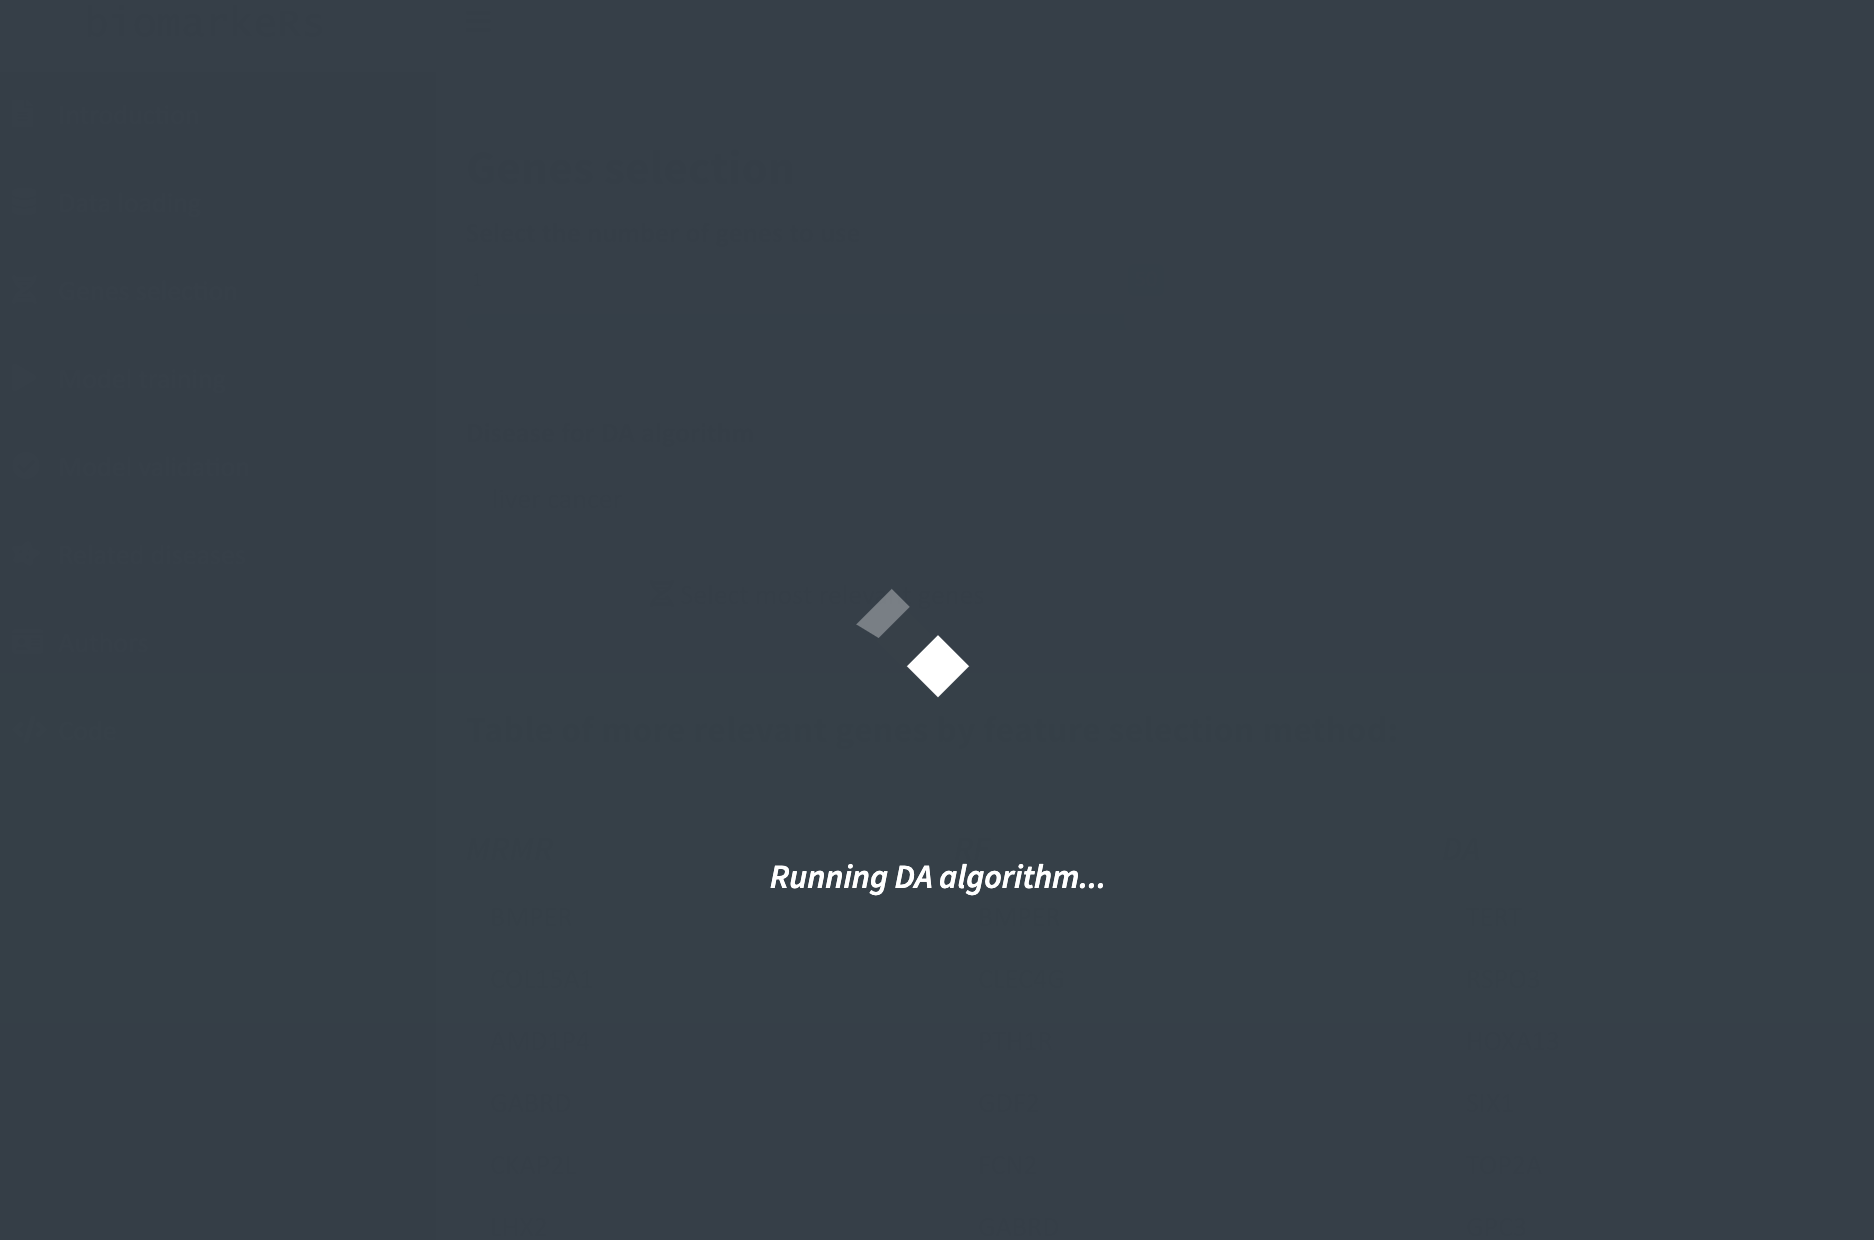
\includegraphics[width=.95\textwidth]{figuras/42_spinner_2.png}
	\end{minipage}%
	\begin{minipage}{.5\textwidth}
		\centering
		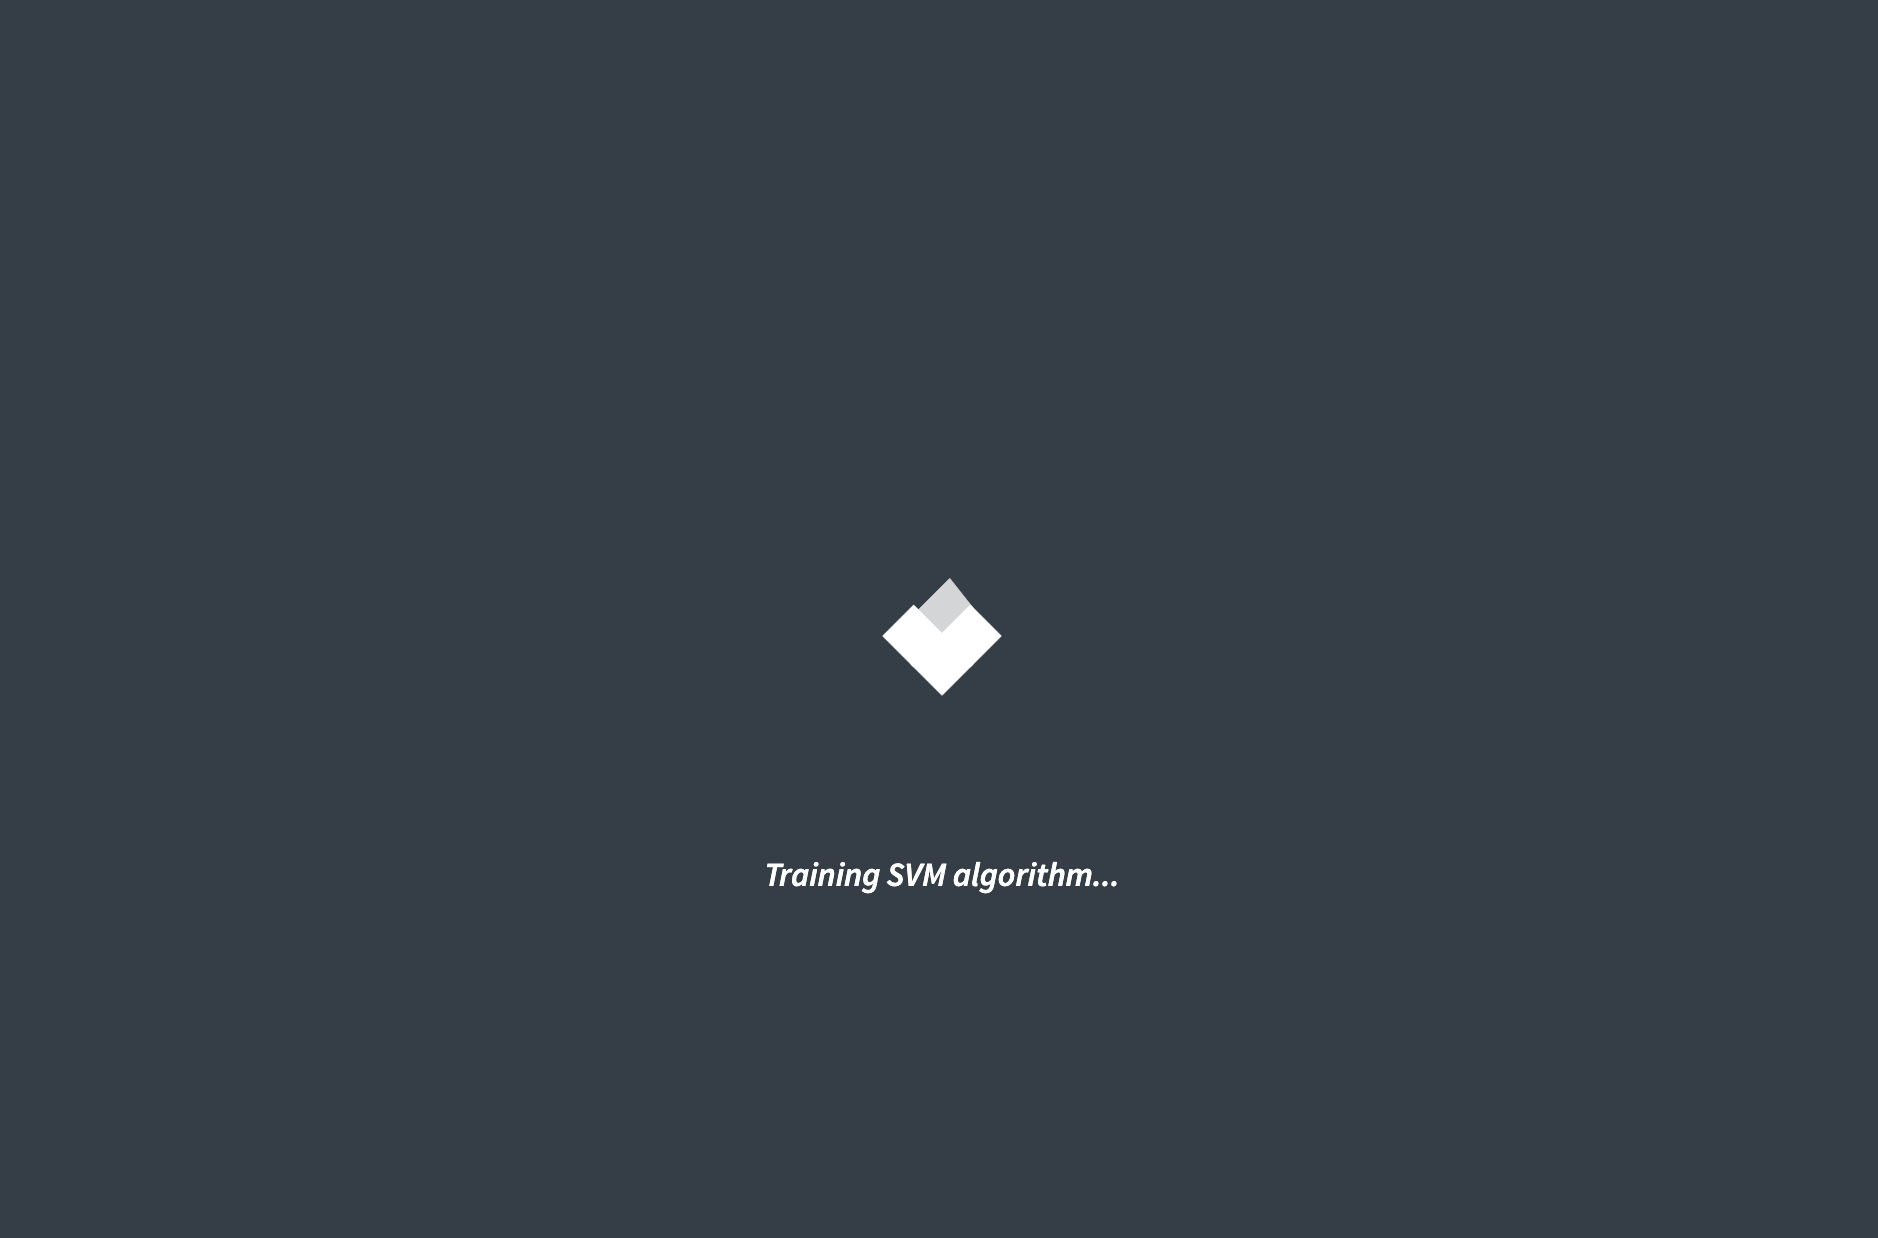
\includegraphics[width=.95\textwidth]{figuras/42_spinner_1.png}
	\end{minipage}
\end{figure}

\end{center}

La aplicación puede ejecutarse de forma local usando RStudio (un entorno de desarrollo integrado de R) \cite{RStudioTeam2020} y también está disponible de forma online en el enlace \url{https://dredondo.shinyapps.io/biomarkeRs/}.\\

El fichero \textit{\texttt{shiny/app.R}} del repositorio de GitHub asociado al trabajo \cite{Redondo-Sanchez2020} contiene el código de R desarrollado para crear la aplicación web.

\section{Utilidades de la aplicación}

A la izquierda de la aplicación se presenta un menú lateral con enlaces a los distintos apartados. A continuación se describen las distintas utilidades de cada apartado.\\

\subsection{Introducción}

En el apartado de introducción (Figura 43) se presenta la aplicación y se muestra el abstract del presente trabajo.

\newpage
\begin{center}
	\textbf{Figura 43}. Apartado de introducción de \texttt{biomarkeRs}.
\end{center}

\begin{center}
	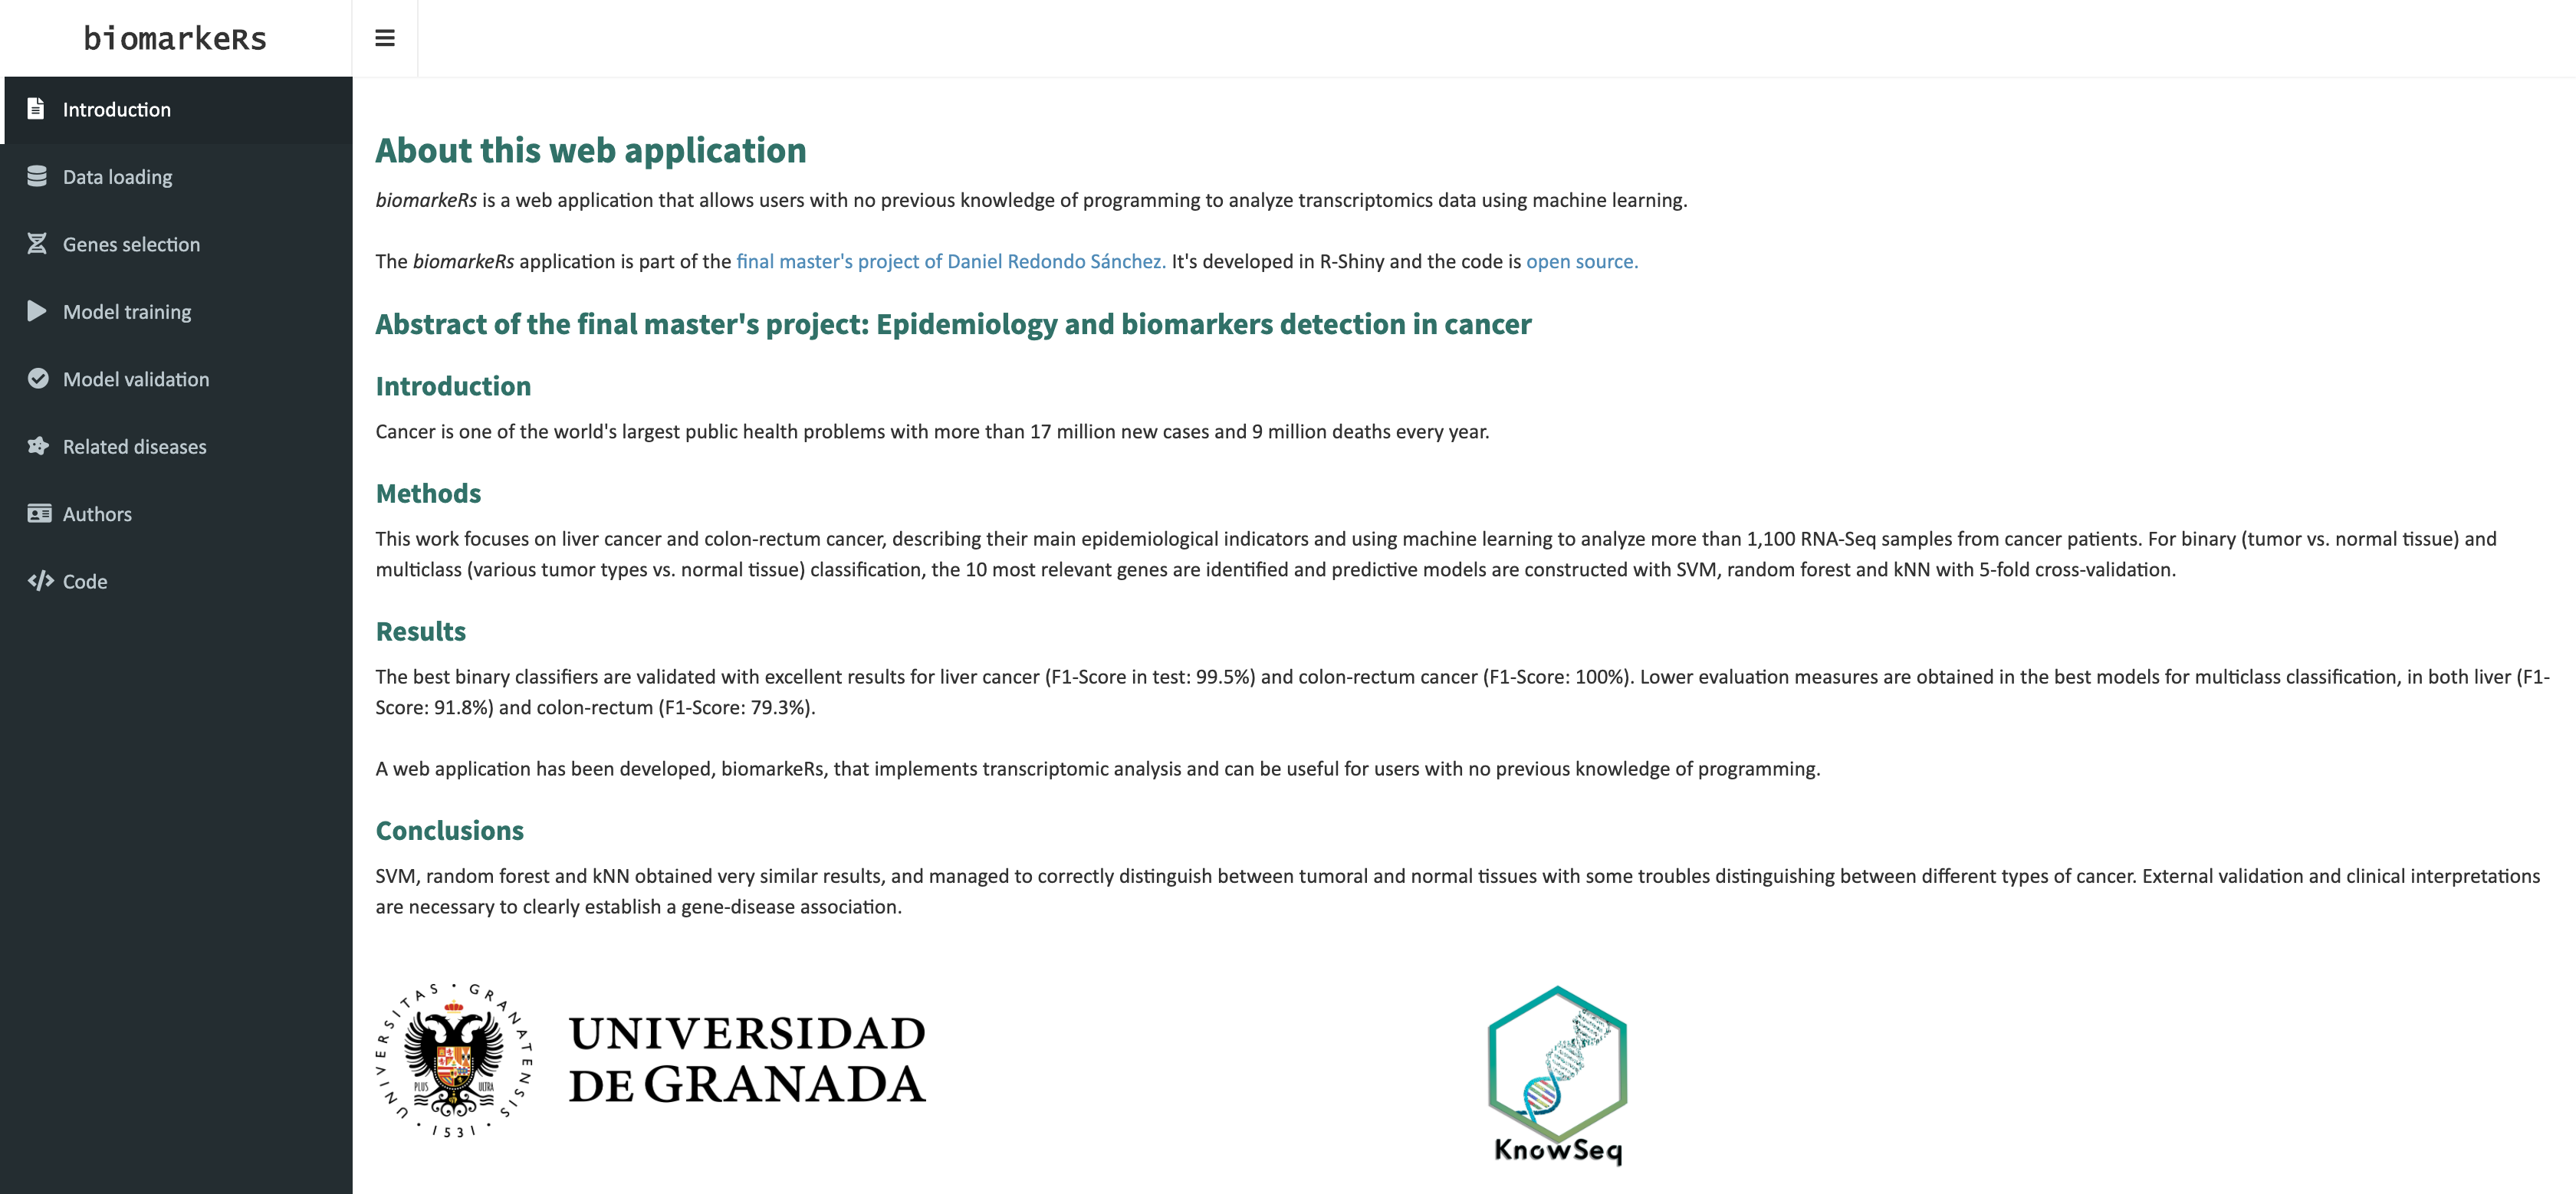
\includegraphics[width=.90\textwidth]{figuras/43_introduction.png} \\
\end{center}

\subsection{Carga de datos}

\begin{center}
	\textbf{Figura 44}. Apartado de carga de datos de \texttt{biomarkeRs}.
\end{center}

\begin{center}
	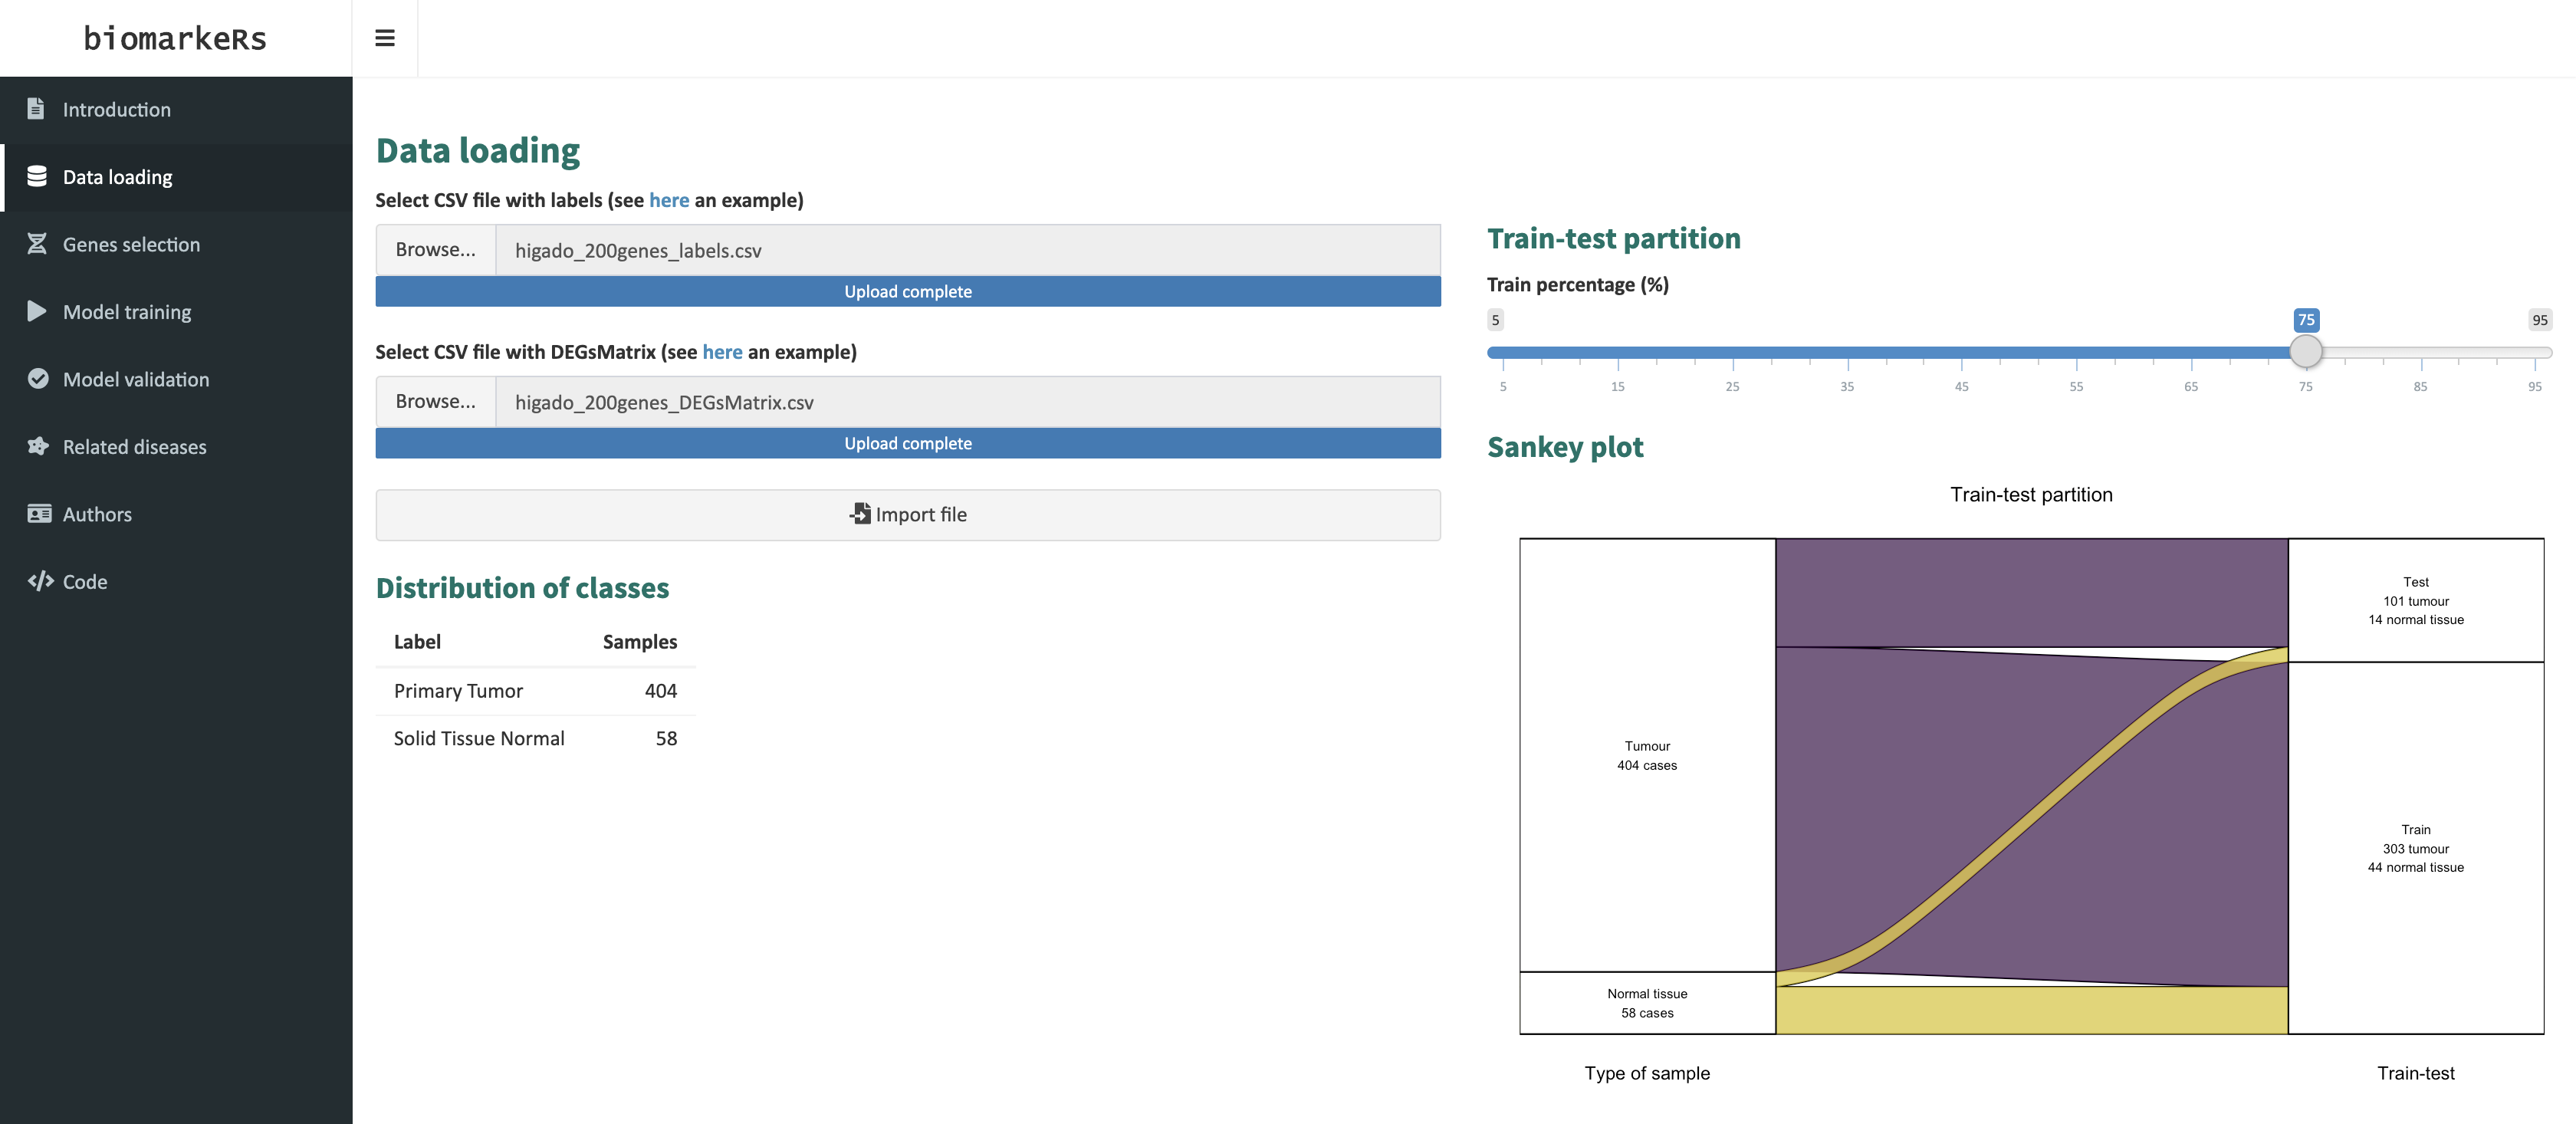
\includegraphics[width=.90\textwidth]{figuras/44_data_loading.png} \\
\end{center}

El apartado de carga de datos (Figura 44) permite al usuario cargar dos ficheros que deben tener formato CSV: uno que contiene las etiquetas de las muestras, y otro que contiene la matriz de expresión de genes de los DEGs encontrados. En la actualidad, la aplicación sólo permite realizar análisis biclase. Además, se han añadido  enlaces para descargar ficheros de ejemplo que están ubicados en el repositorio de GitHub del trabajo \cite{Redondo-Sanchez2020}. Los ficheros de ejemplo utilizan el conjunto de datos de cáncer de hígado empleado en el capítulo 4.\\

Para facilitar la rápida ejecución de la aplicación, los ficheros de ejemplo se han creado limitando el número de DEGs a 200 genes usando el parámetro \textit{\texttt{number}} de \textit{\texttt{KnowSeq::DEGsExtraction}}. También se han creado ficheros sin limitar el número de DEGs, con la misma condición para extracción de DEGs que la considerada para el capítulo 4 (p-valor de p = 0,001). Estos ficheros de ejemplo se pueden encontrar en \textit{\texttt{shiny/datos}} del repositorio de GitHub \cite{Redondo-Sanchez2020}. Además, el código que genera los ficheros de ejemplo a partir de los datos originales está disponible en el fichero \textit{\texttt{shiny/create\_data\_examples.R}}.\\

Una vez cargados los datos, se obtiene una tabla con la frecuencia de las distintas clases. En la parte derecha de la aplicación se ubica un control deslizante para personalizar el porcentaje de datos que se usa para crear los conjuntos de entrenamiento y test. Debajo de este control, un diagrama de Sankey muestra el reparto de las clases en los conjuntos de entrenamiento y test. El gráfico se actualiza automáticamente al cambiar el porcentaje del reparto.

\subsection{Selección de genes}

\begin{center}
	\textbf{Figura 45}. Apartado de selección de genes de \texttt{biomarkeRs}.
\end{center}

\begin{center}
	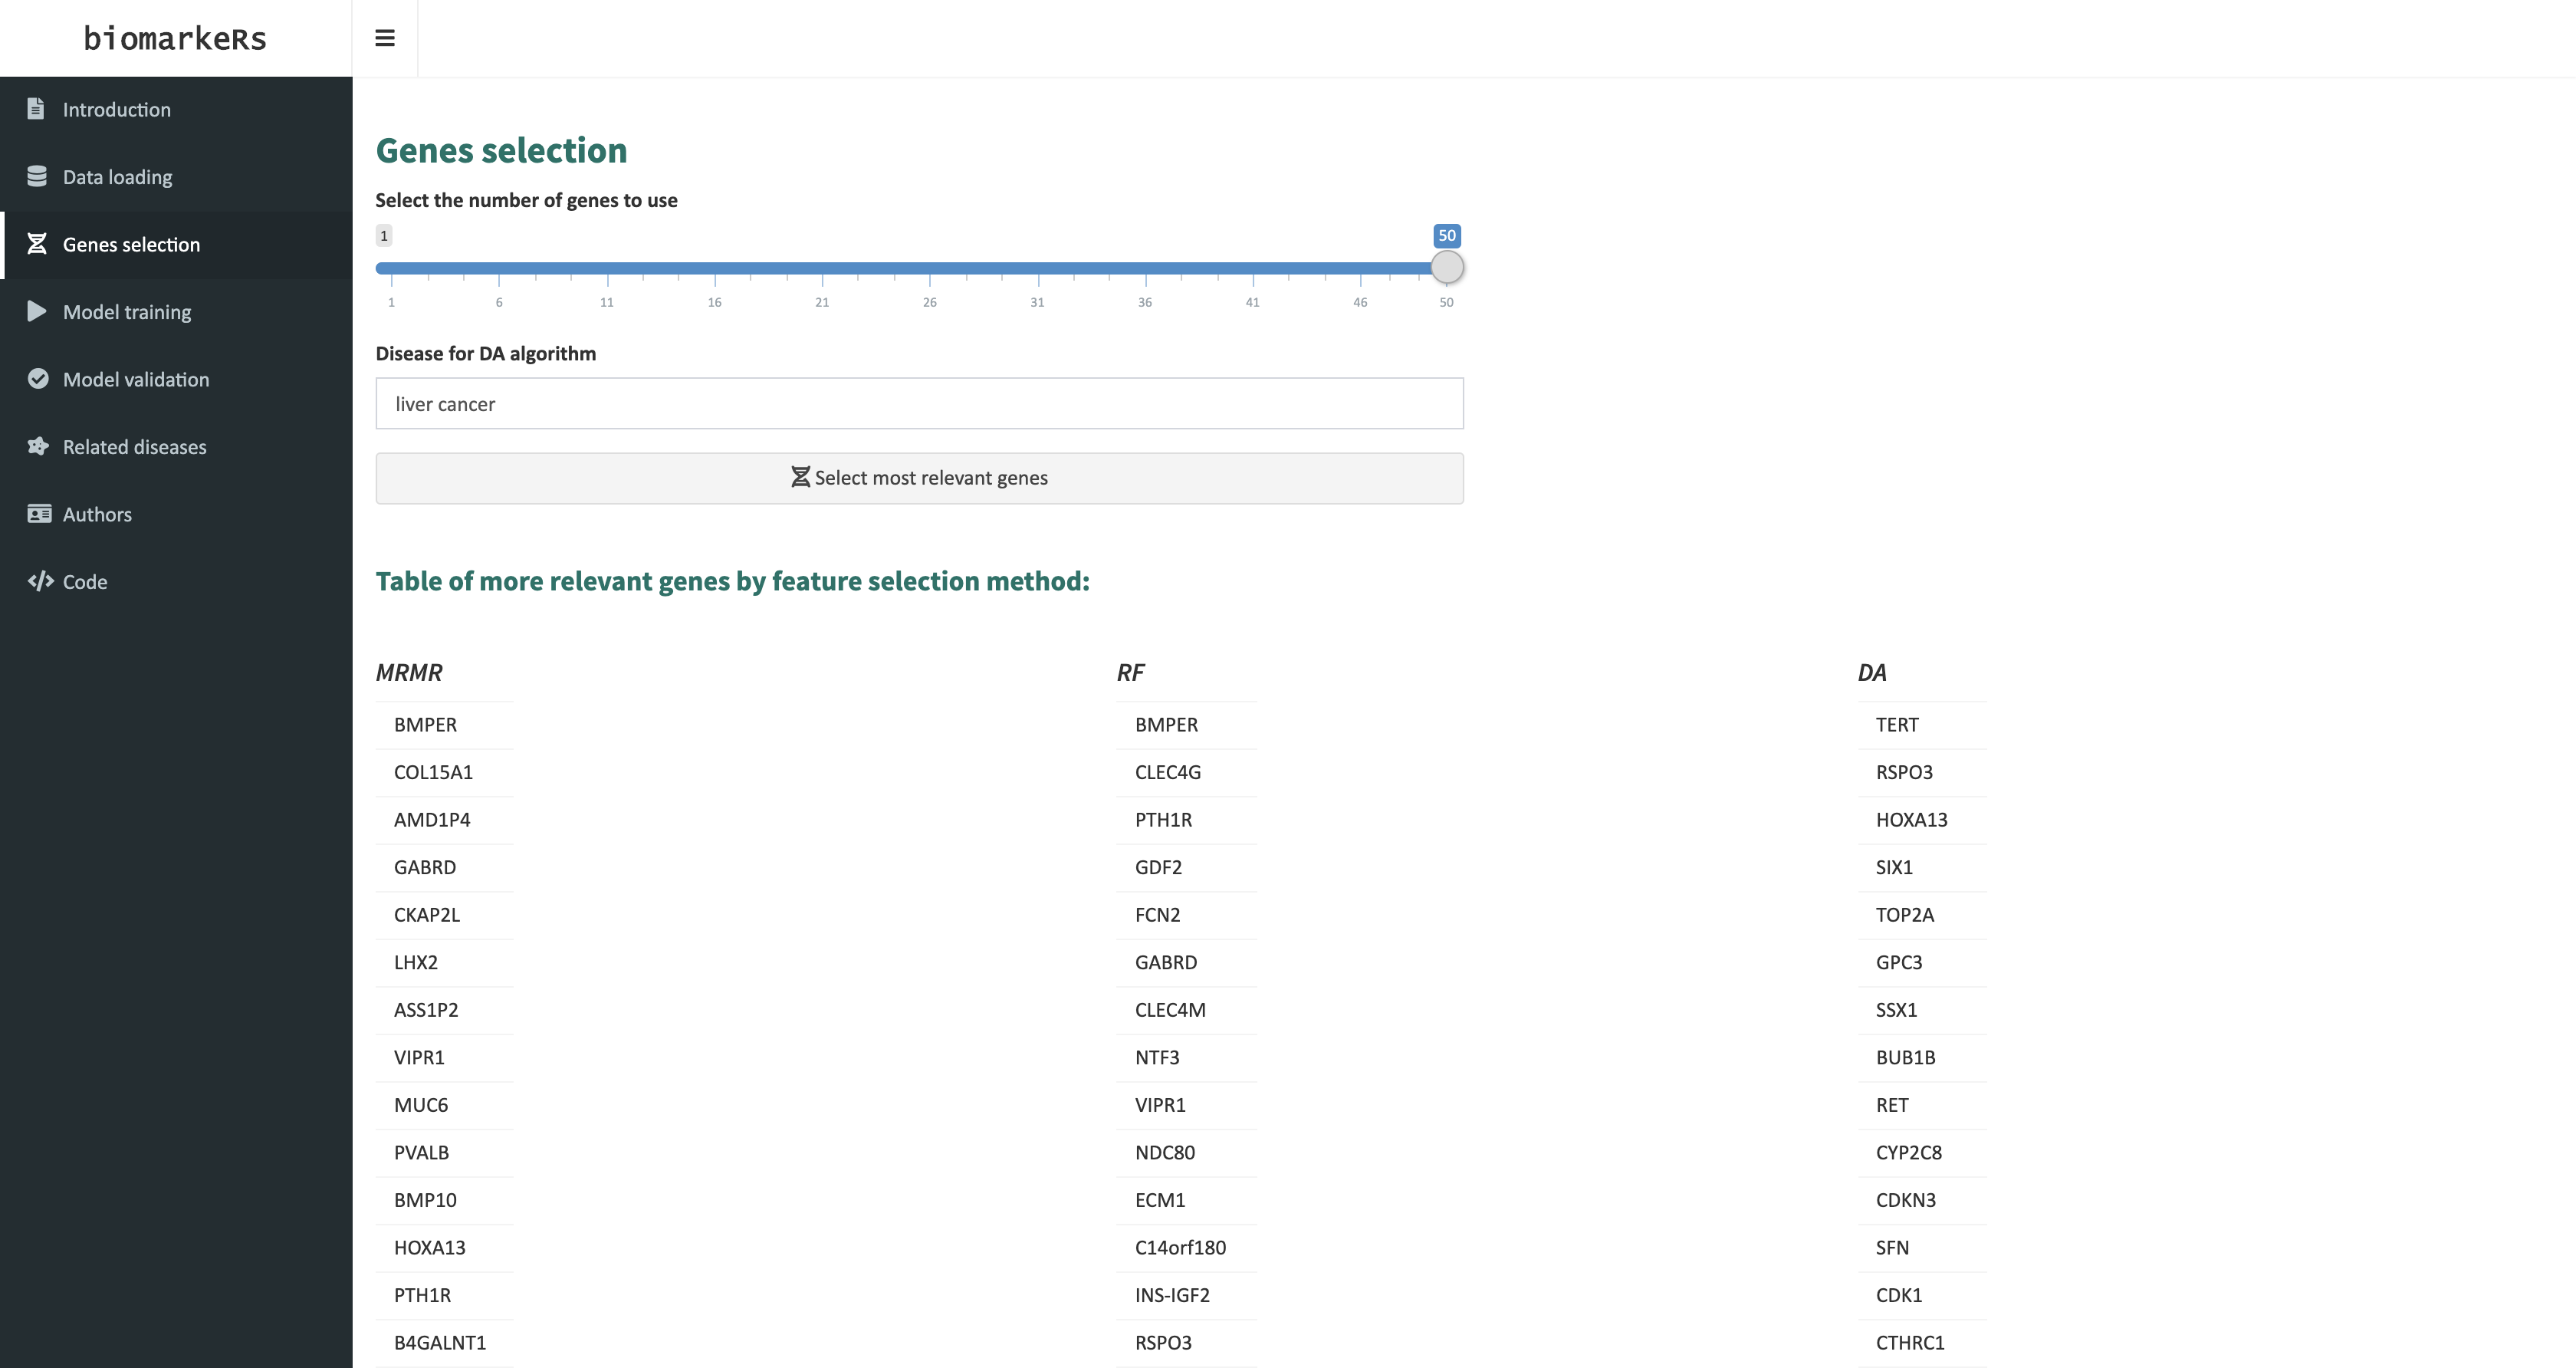
\includegraphics[width=.90\textwidth]{figuras/45_genes_selection.png} \\
\end{center}

Tras cargar los datos en el apartado anterior, en este apartado (Figura 45) la aplicación encuentra biomarcadores según tres métodos de selección de características: mRMR, RF y DA. La aplicación permite seleccionar hasta 50 genes, y para el método DA hay un campo de texto libre para escribir la enfermedad con la que se está trabajando. Los genes encontrados se muestran en una tabla con una columna para cada método de selección de características.

\subsection{Entrenamiento de modelos}

\begin{center}
	\textbf{Figura 46}. Apartado de entrenamiento de modelos de \texttt{biomarkeRs}.
\end{center}

\begin{center}
	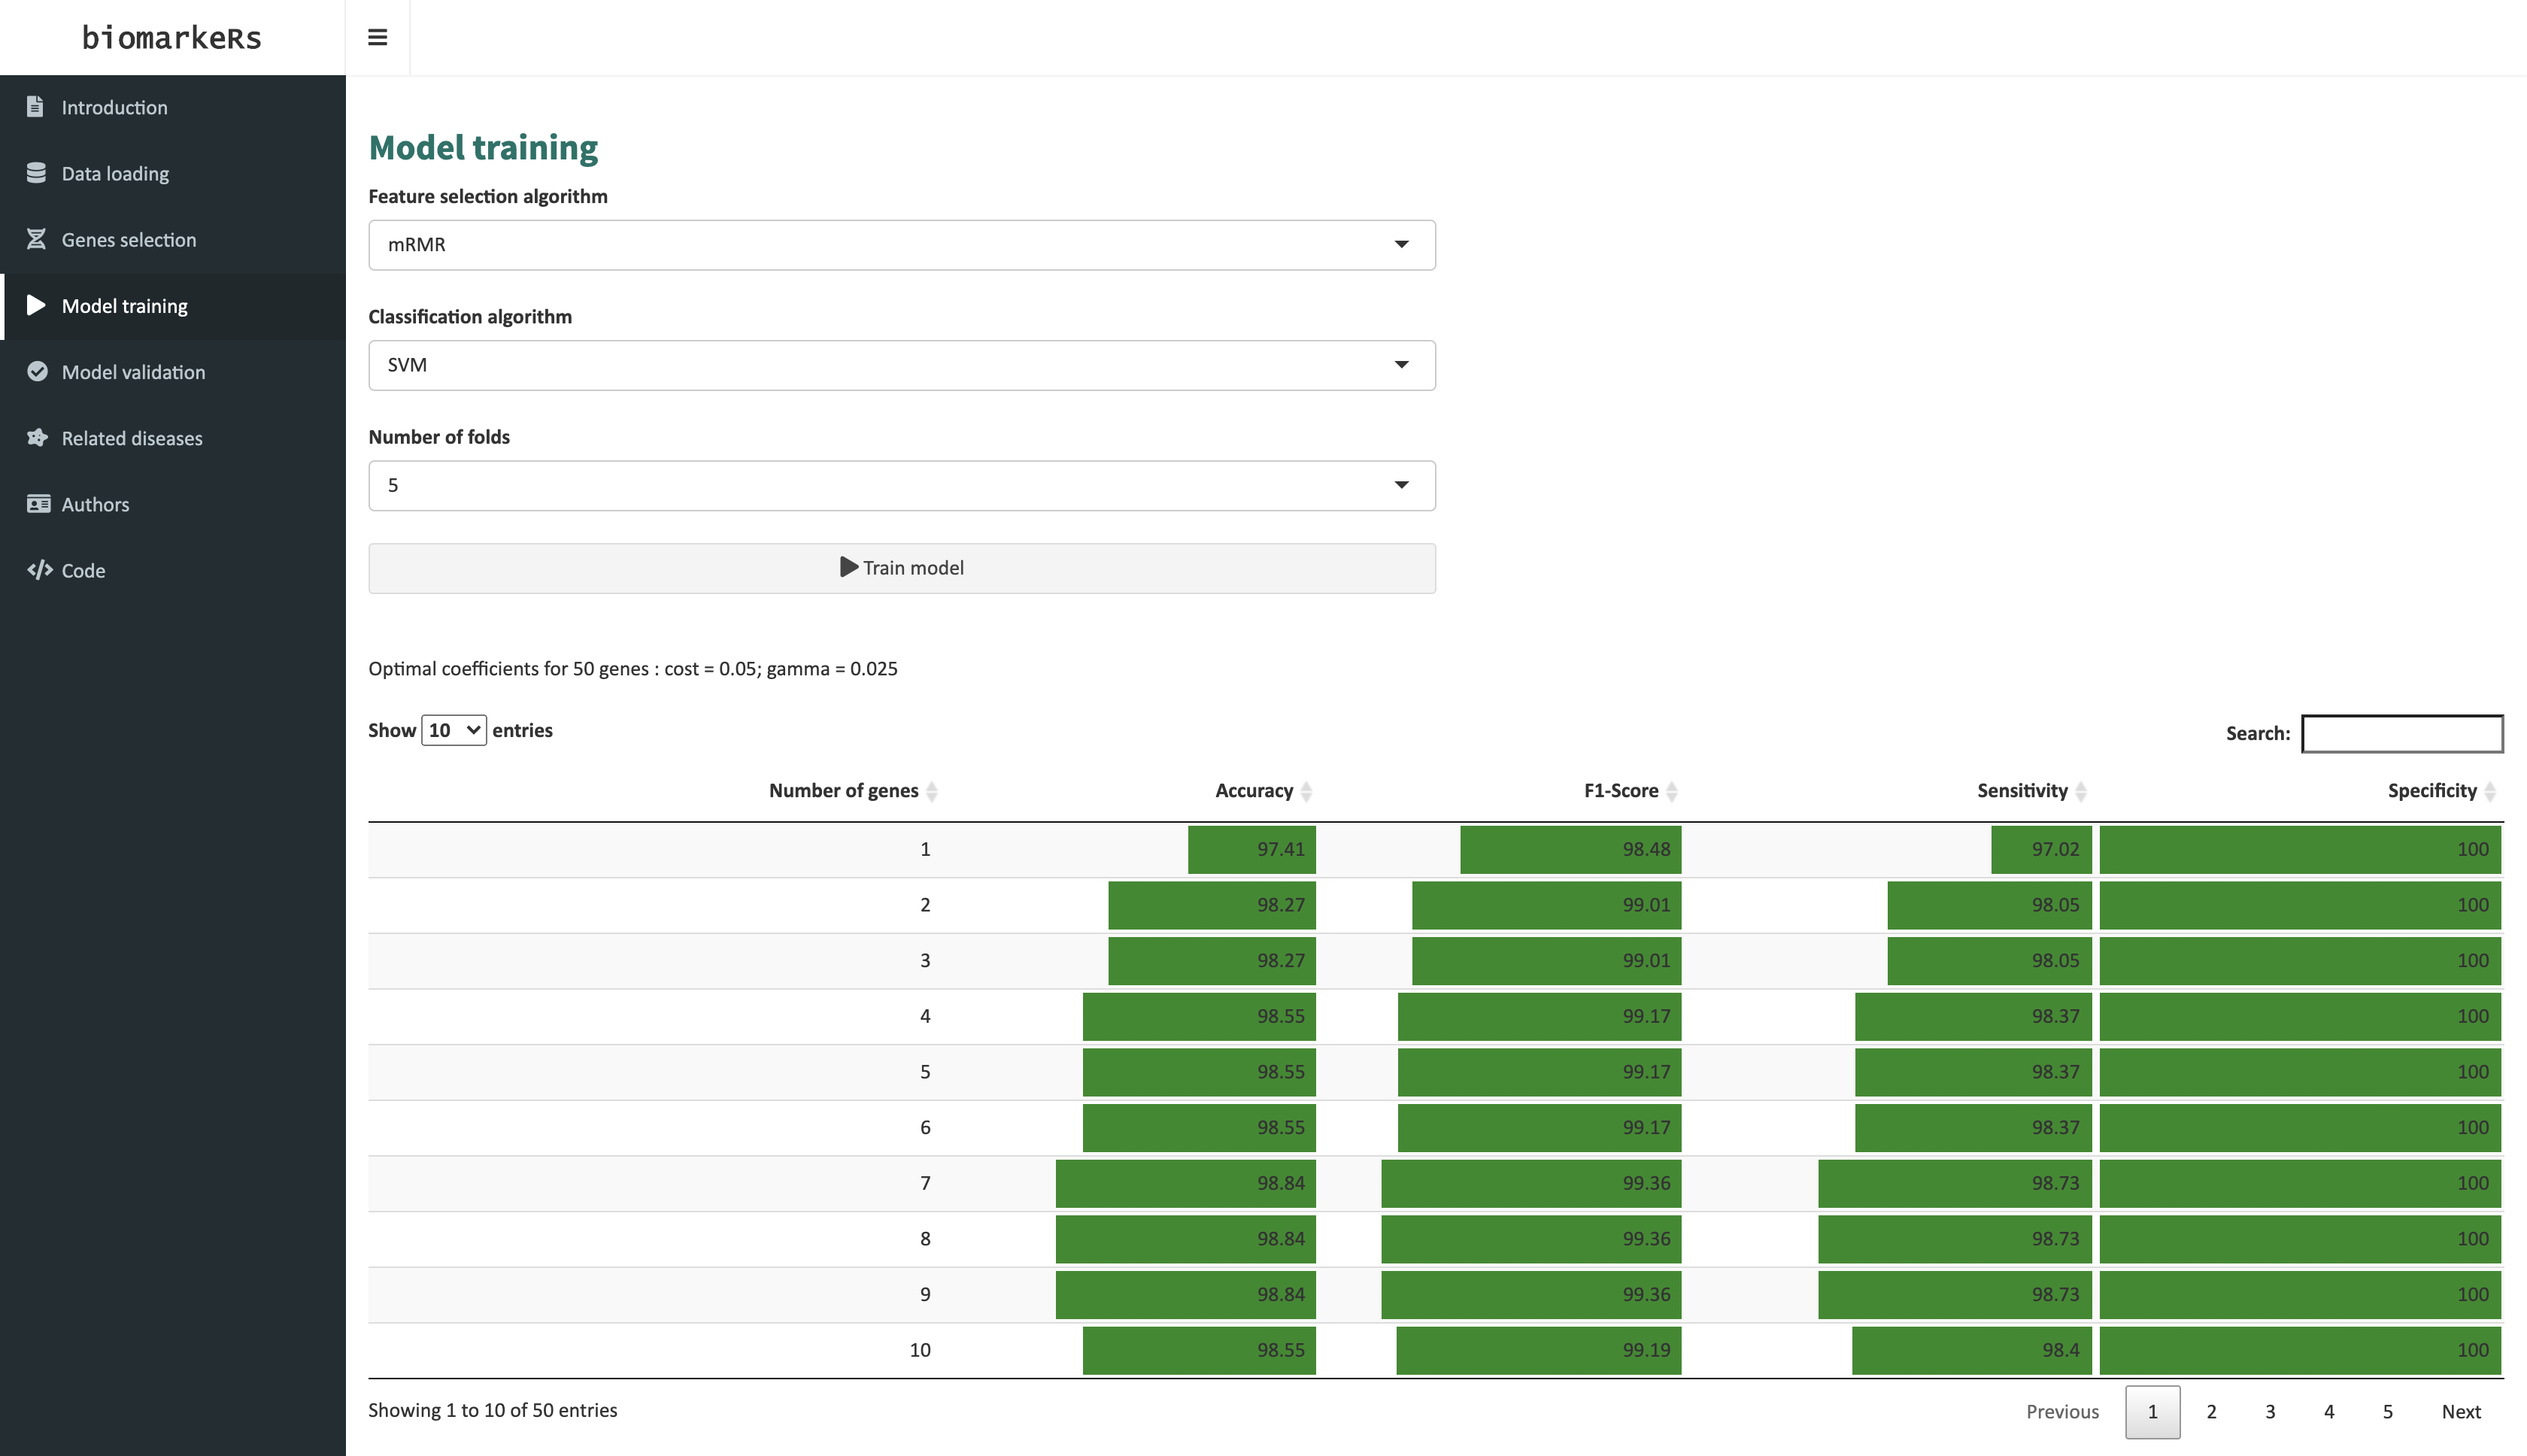
\includegraphics[width=.90\textwidth]{figuras/46_model_training.png} \\
\end{center}

En este apartado (Figura 46) se entrenan modelos en base a tres parámetros que se eligen de listas desplegables:
\begin{itemize}
	\item Método de selección de características. Puede ser mRMR, RF o DA.
	\item Algoritmo de clasificación. Puede ser SVM, RF o kNN.
	\item Número de folds. Puede ser 3, 5 ó 10.
\end{itemize}

Tras hacer clic en el botón, se muestran los resultados de precisión, F1-Score, sensibilidad y especificidad para cada número de genes. Estos indicadores se muestran en una tabla interactiva que permite ordenar de forma ascendente o descendente por cualquier columna, para hallar rápidamente los mejores valores de cada indicador. Además del valor obtenido, cada celda de la tabla tiene incluido un gráfico de barras para visualizar de forma sencilla la evolución de los distintos indicadores. Finalmente, para SVM y kNN se muestran encima de la tabla los parámetros óptimos obtenidos.

\subsection{Validación de modelos}

\begin{center}
	\textbf{Figura 47}. Apartado de validación de modelos de \texttt{biomarkeRs}.
\end{center}

\begin{center}
	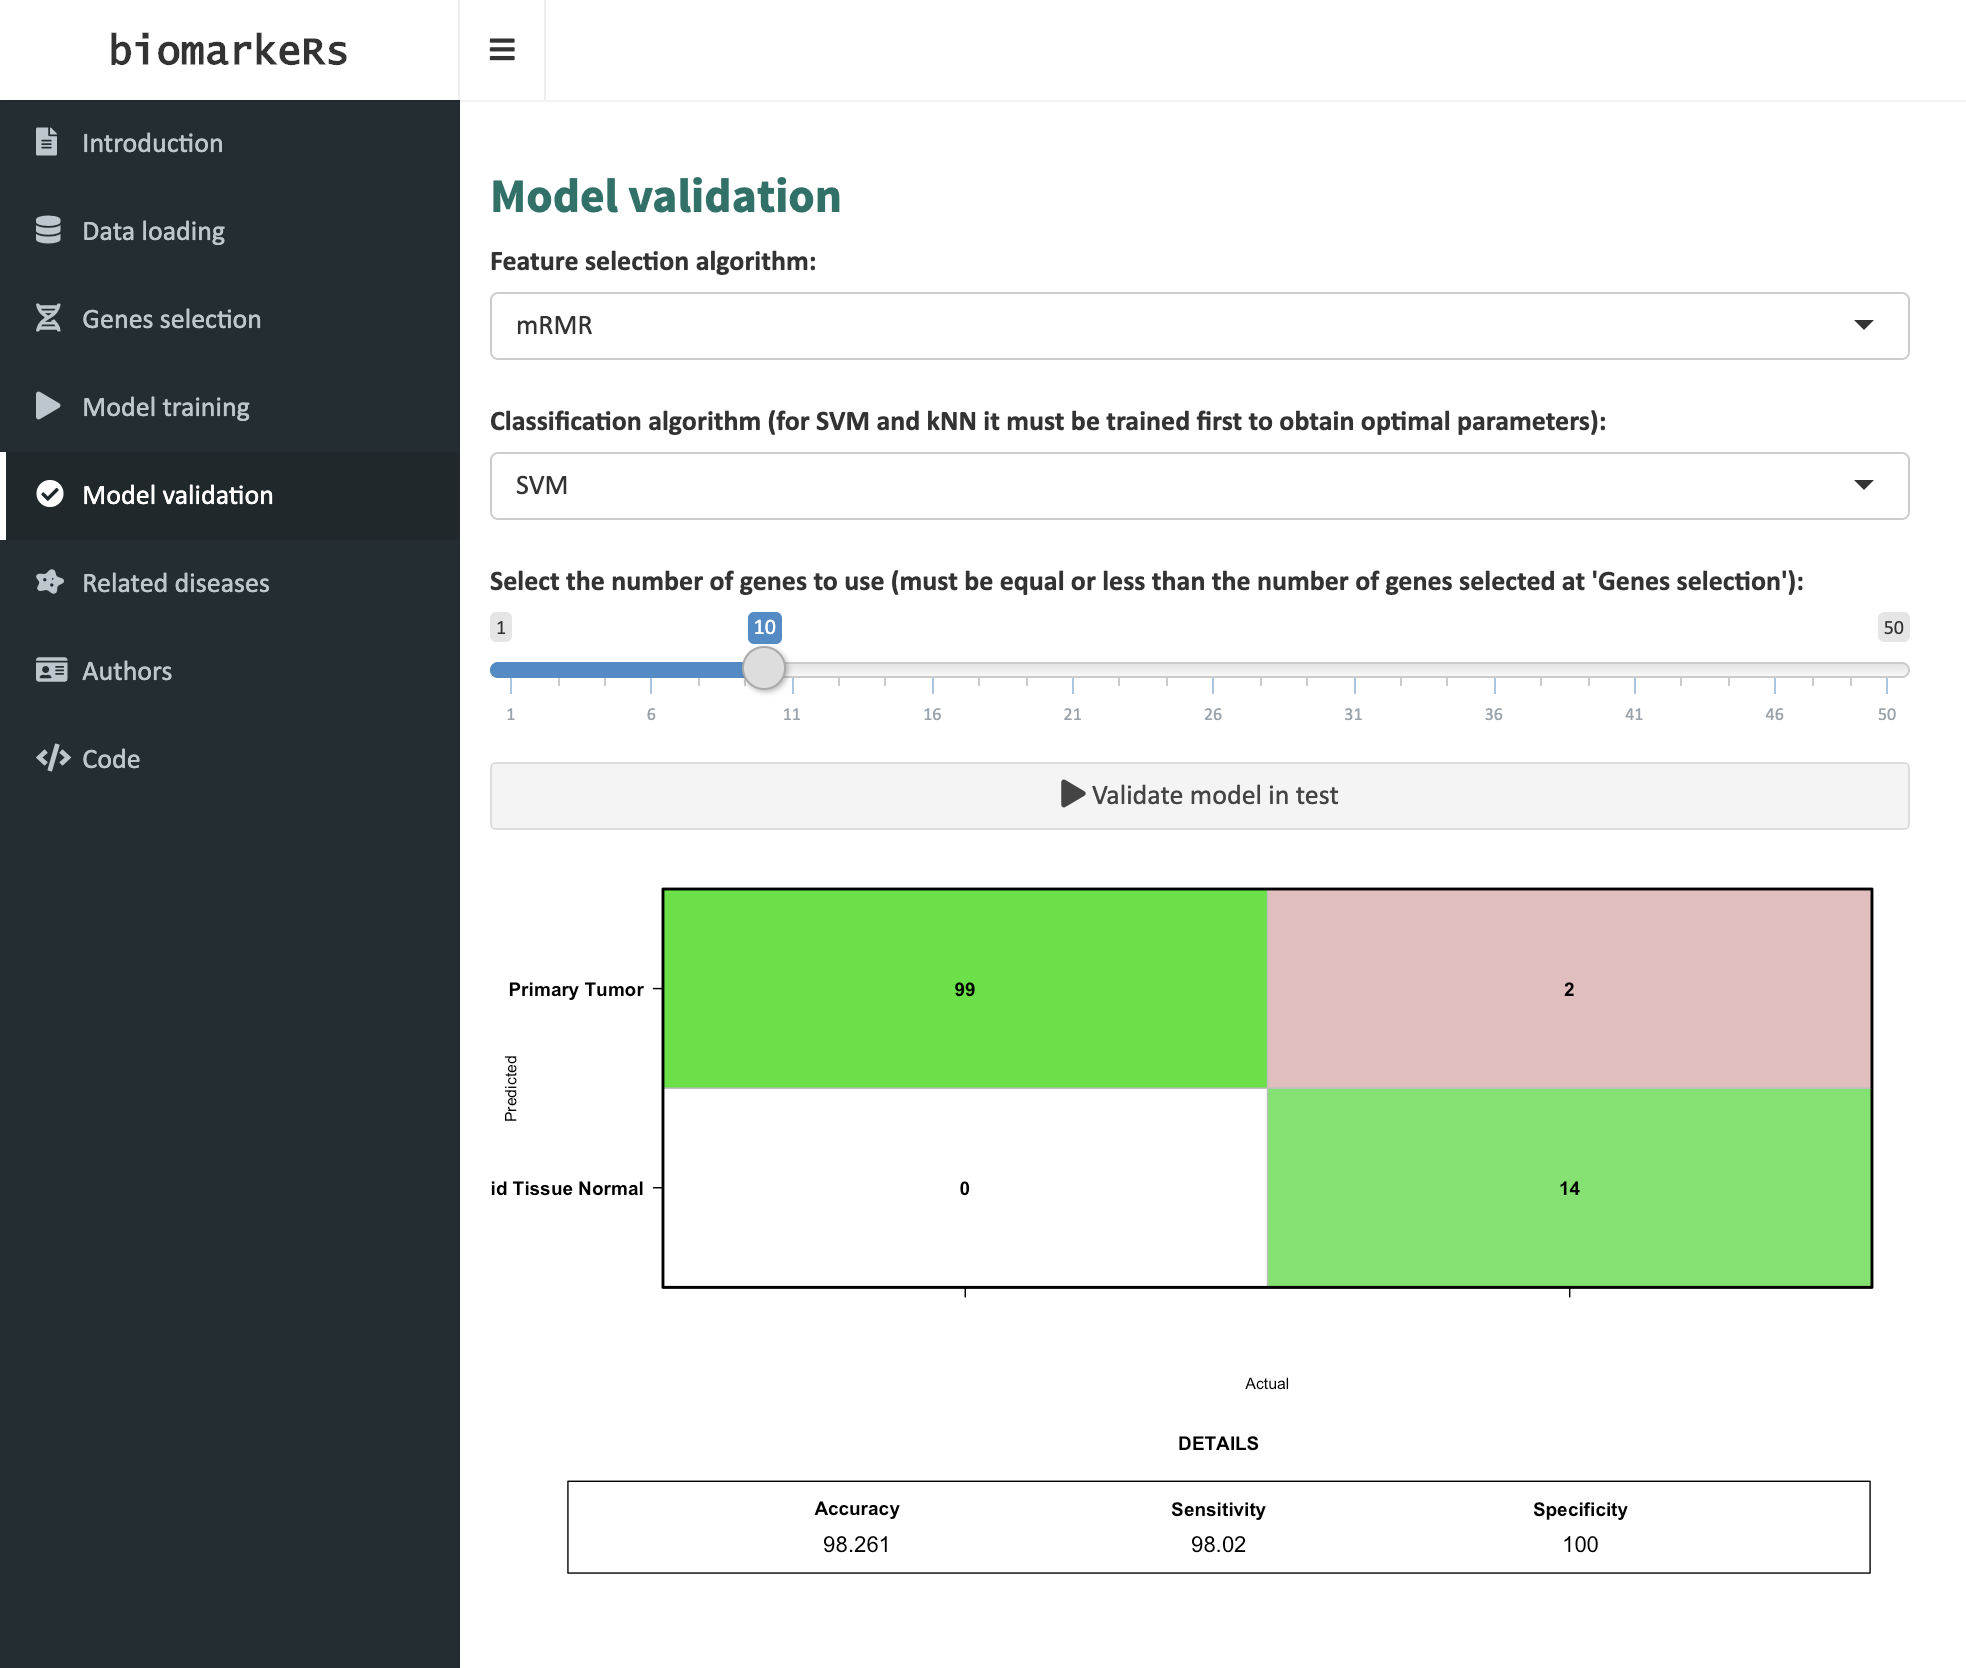
\includegraphics[width=.90\textwidth]{figuras/47_model_validation.png} \\
\end{center}

Una vez explorado el entrenamiento de modelos, en este apartado se pueden validar modelos en el conjunto de test (Figura 47). En este caso hay que seleccionar un método de selección de características (mRMR/RF/DA) y un algoritmo de clasificación (SVM/RF/kNN), así como el número de genes a usar. Tras hacer clic en el botón, se muestra de forma gráfica la matriz de confusión obtenida, así como los valores de precisión, sensibilidad y especificidad.

\newpage
\subsection{Enfermedades relacionadas}

Este apartado (Figura 48) permite conocer la evidencia científica existente sobre las enfermedades relacionadas con un gen en concreto. Tras especificar el nombre del gen, se obtiene una tabla interactiva donde cada fila es una enfermedad relacionada. Las primera columna muestra el nombre de la enfermedad, y el resto de columnas un coeficiente que mide el nivel de asociación según distintos tipos de evidencia (general, literatura, expresión de RNA, genética, mutaciones somáticas, fármacos, animales y rutas metabólicas). Los coeficientes se obtienen de la plataforma \textit{Open Targets} \cite{OpenTargets2020} y varían entre 0 (ninguna evidencia) y 1 (evidencia total).

\begin{center}
	\textbf{Figura 48}. Apartado de enfermedades relacionadas de \texttt{biomarkeRs}.
\end{center}

\begin{center}
	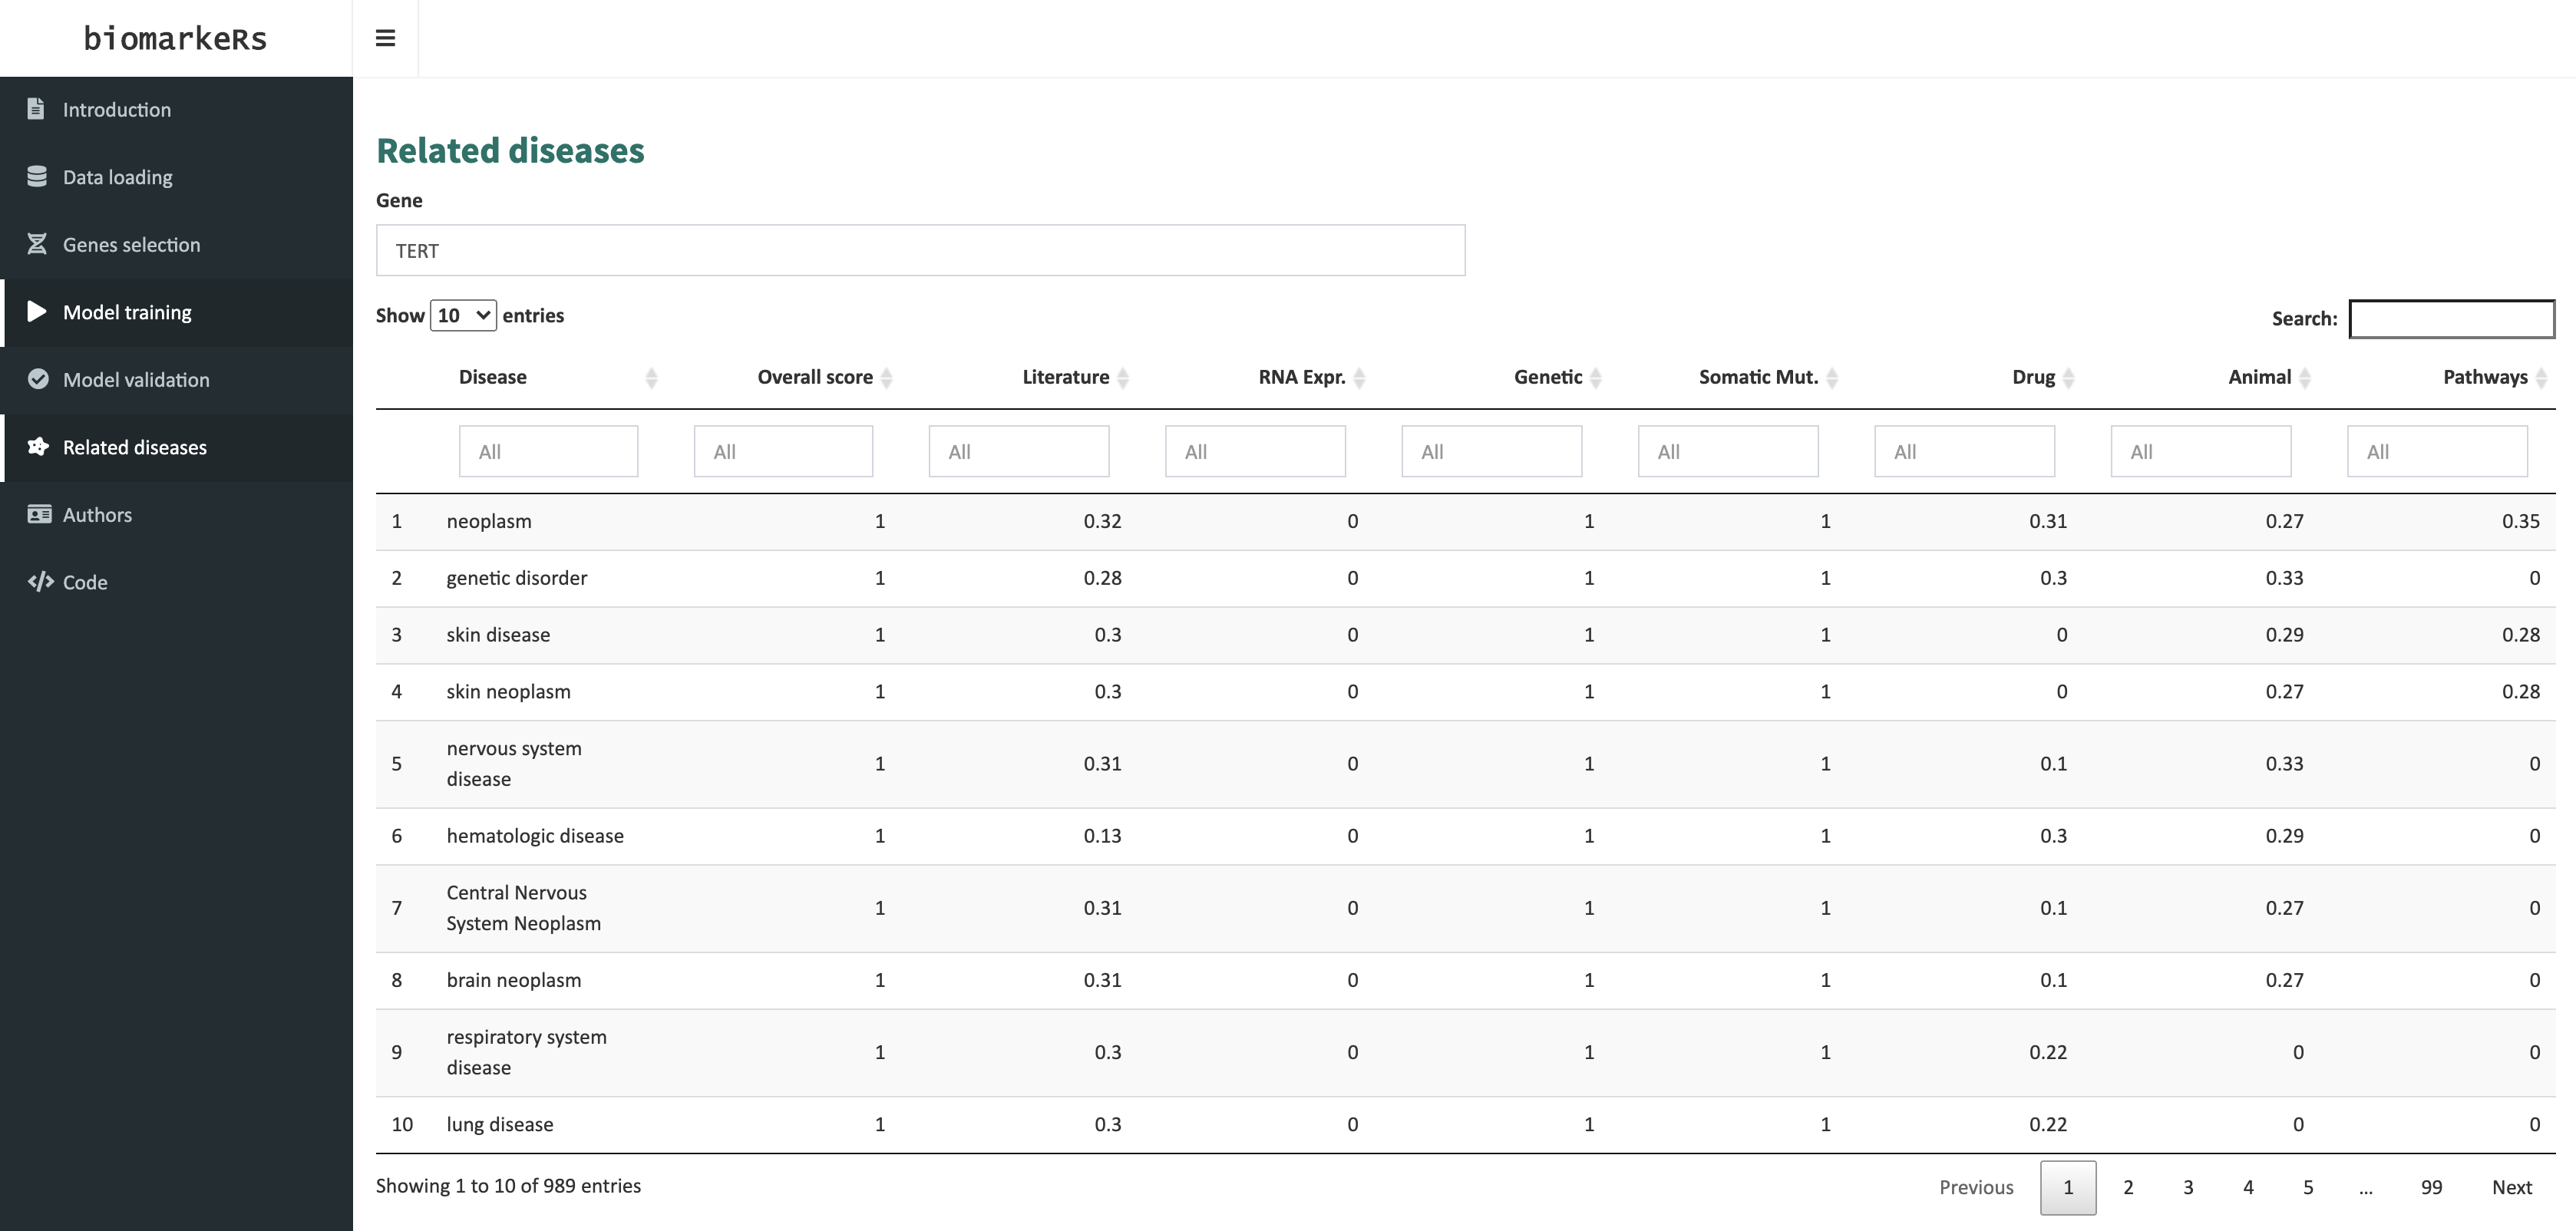
\includegraphics[width=.90\textwidth]{figuras/48_related_diseases.png} \\
\end{center}

La tabla interactiva tiene muchas funcionalidades que facilita la comprensión de los resultados:
\begin{itemize}
	\item Permite ordenar las columnas de forma ascendente y descendente.
	\item Permite filtrar las enfermedades por texto (Figura 49).  Al hacer clic en el campo en blanco debajo de la primera columna, el usuario puede escribir texto libre para encontrar enfermedades relacionadas con algún término concreto.
	\item Permite filtrar las enfermedades por los coeficientes de evidencia. Al hacer clic en el campo en blanco debajo de las columnas, aparece un control deslizante para que el usuario pueda seleccionar cualquier rango.
\end{itemize}

\begin{center}
	\textbf{Figura 49}. Enfermedades relacionadas con el gen TERT que contienen la palabra hígado (\textit{liver}).
\end{center}

\begin{center}
	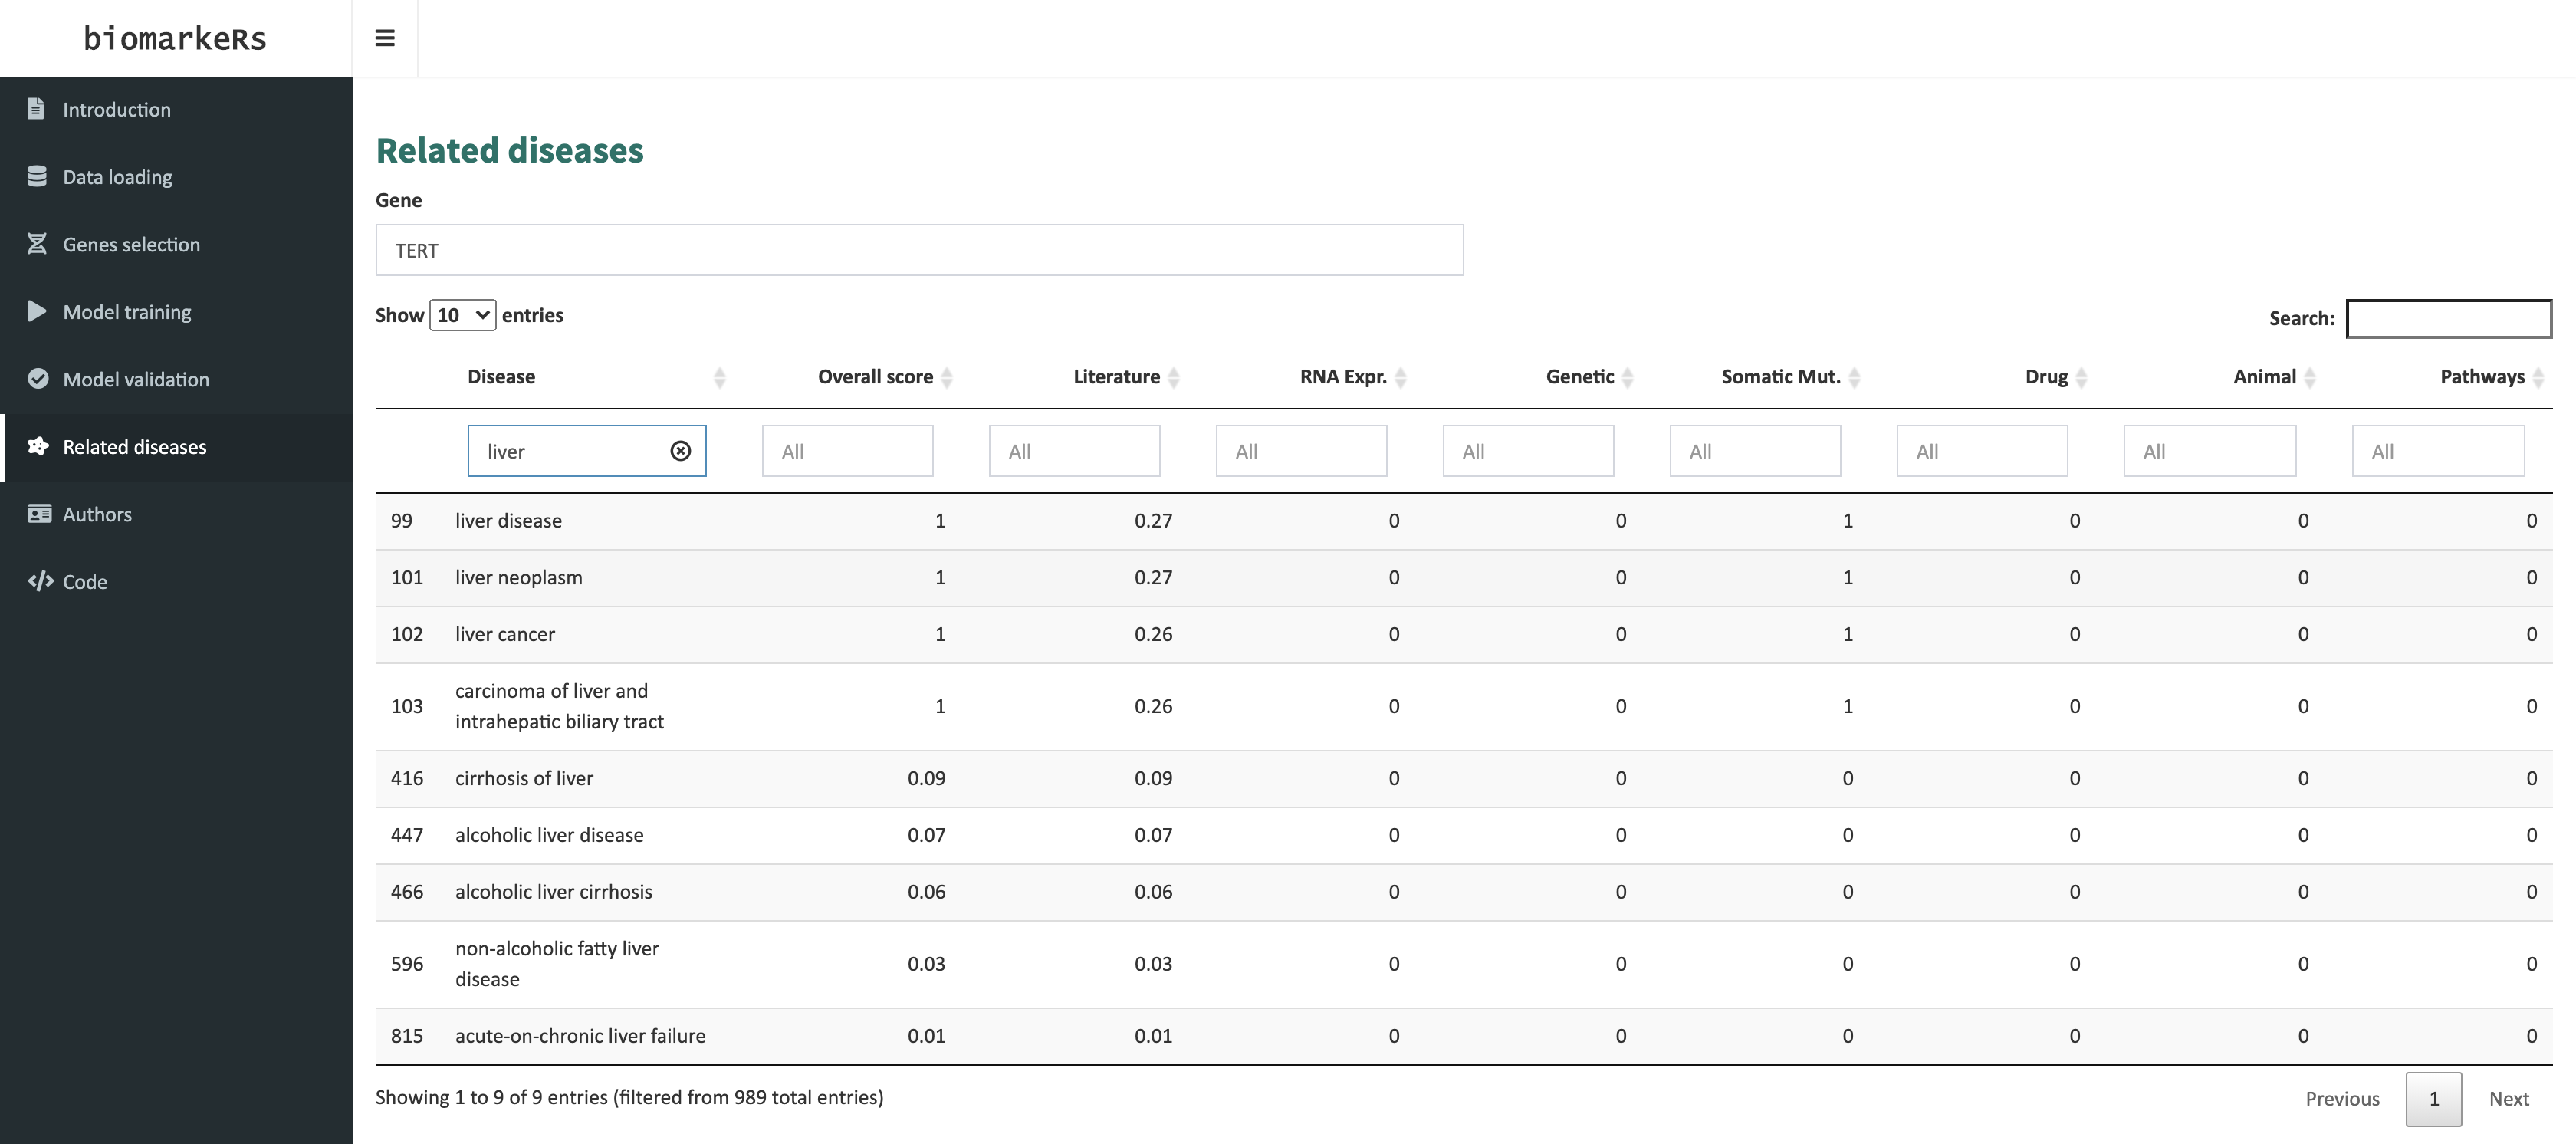
\includegraphics[width=.90\textwidth]{figuras/49_related_diseases_filtered.png} \\
\end{center}

\subsection{Autores}

En este apartado (Figura 50) se muestran los autores de la aplicación. Se ha añadido además una sección de contacto para resolver dudas de usuarios, recibir sugerencias con mejoras o ser informados de fallos encontrados en la aplicación.

\begin{center}
	\textbf{Figura 50}. Apartado de autores de \texttt{biomarkeRs}.
\end{center}

\begin{center}
	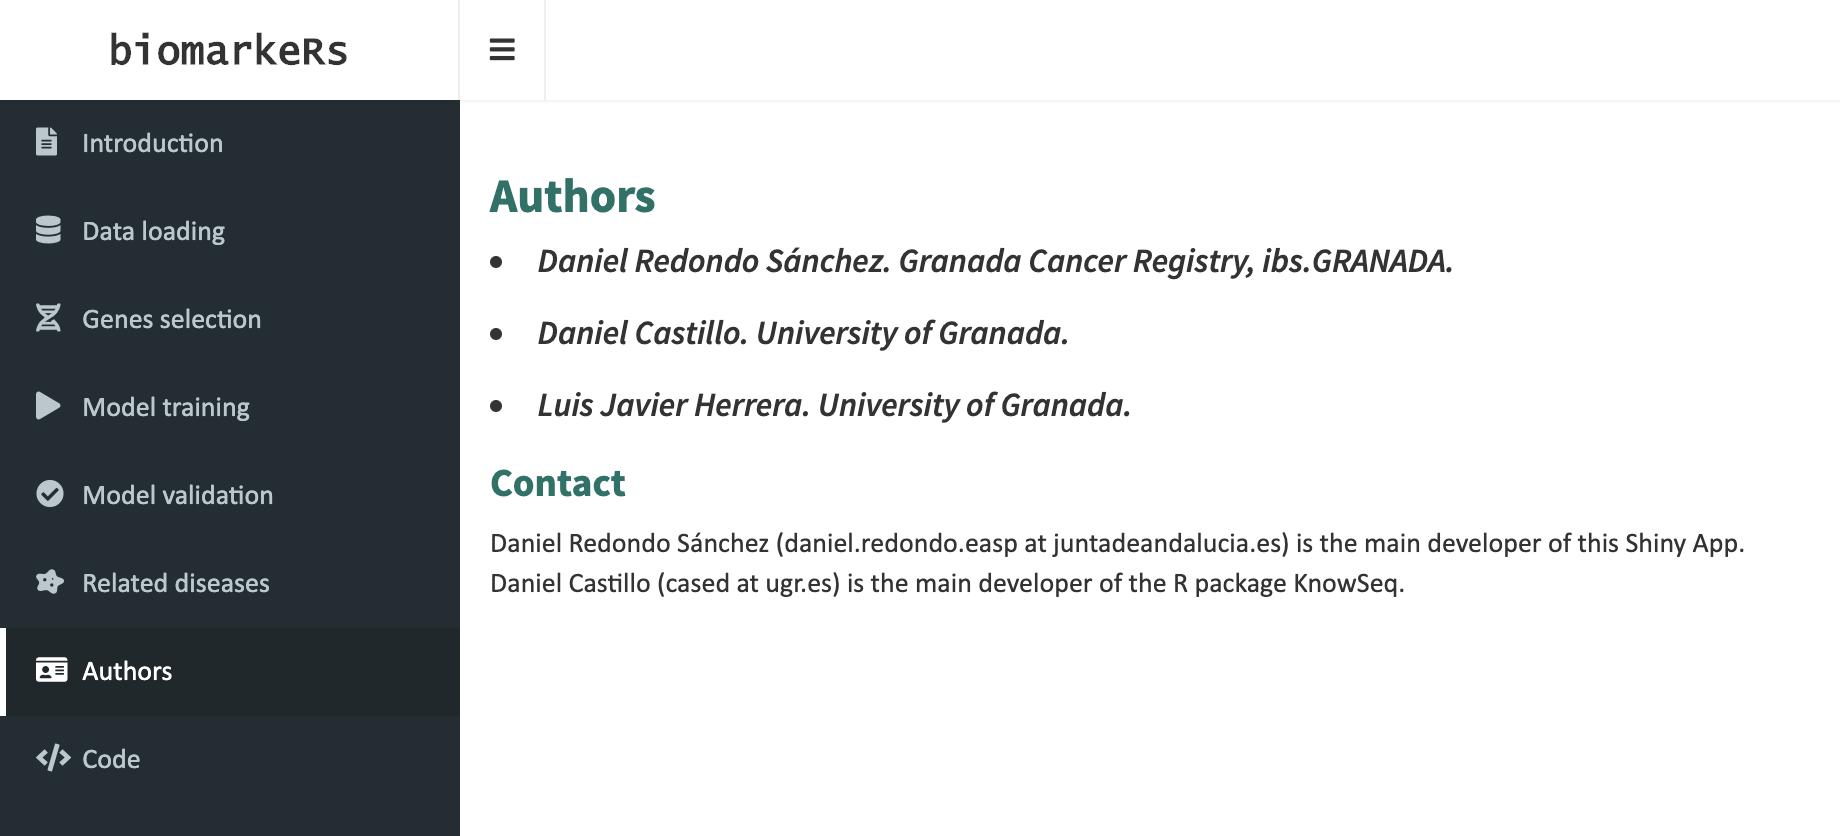
\includegraphics[width=.90\textwidth]{figuras/50_authors.png} \\
\end{center}

\subsection{Código}

En este apartado (Figura 51) se incluye un enlace al repositorio de GitHub del trabajo, donde está disponible el código completo de la aplicación.

\begin{center}
	\textbf{Figura 51}. Apartado de código  de \texttt{biomarkeRs}.
\end{center}

\begin{center}
	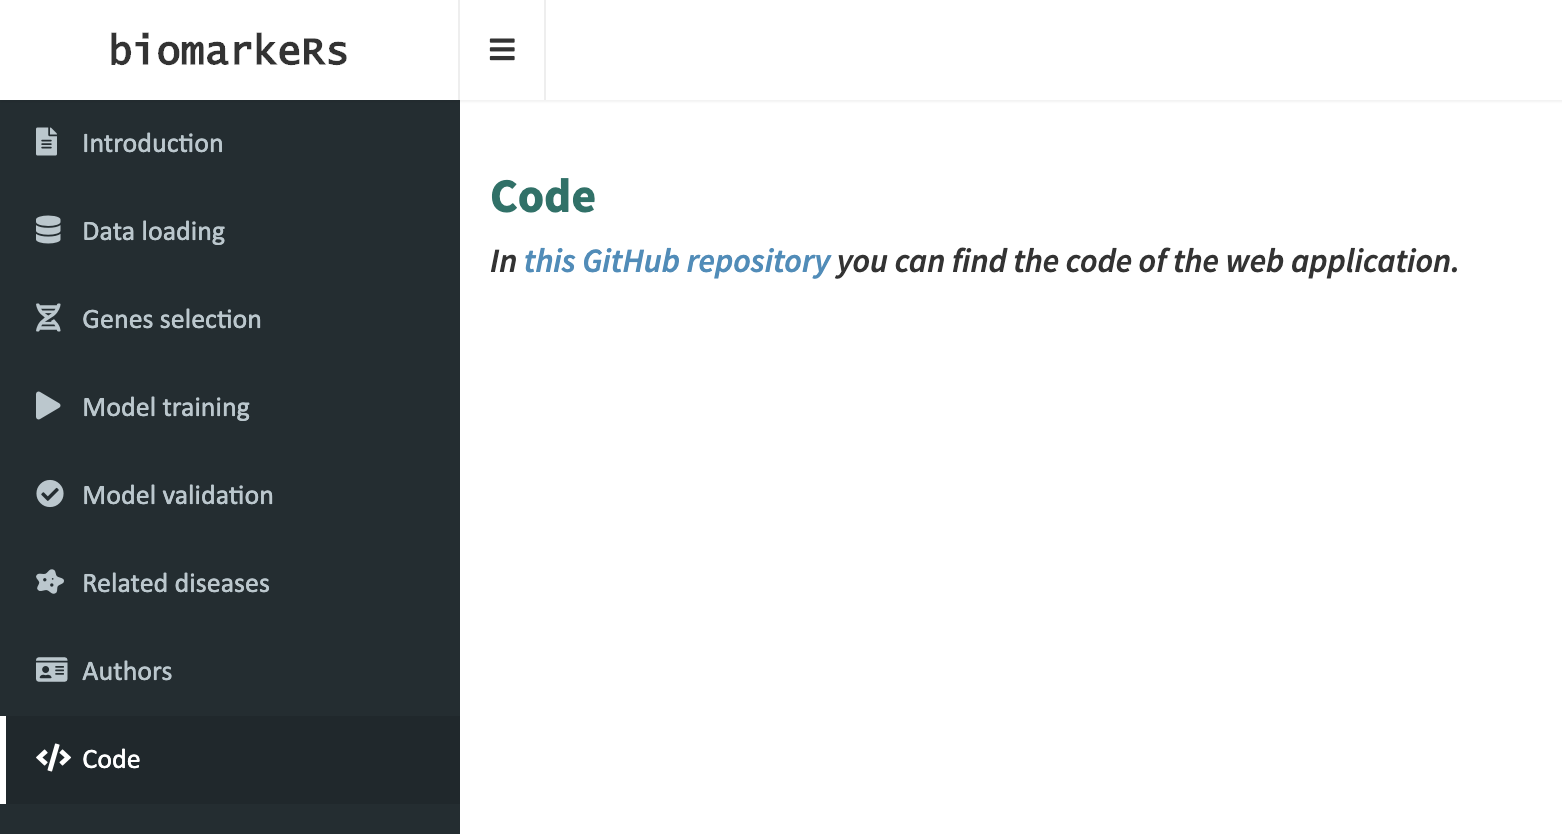
\includegraphics[width=.80\textwidth]{figuras/51_code.png} \\
\end{center}

\section{Características de las versiones web y local}

Las versiones web y local de la aplicación comparten el mismo código fuente, pero en función del uso que se vaya a hacer puede resultar más conveniente usar una versión u otra.\\

La versión web está alojada en \url{https://www.shinyapps.io/}, una plataforma de RStudio que permite la rápida integración de Shiny en una página web. La principal ventaja de esta versión es su accesibilidad mediante cualquier navegador, ya que no es necesaria ninguna instalación previa. Además, se puede acceder también desde cualquier dispositivo móvil sin pérdida de funcionalidades (Figura 52).\\

\newpage
\begin{center}
	\textbf{Figura 52}.  \texttt{biomarkeRs} ejecutándose en dos móviles (iPhone 10, HUAWEI P smart).

	\begin{figure}[H]
		\centering
		\begin{minipage}{.5\textwidth}
			\centering
			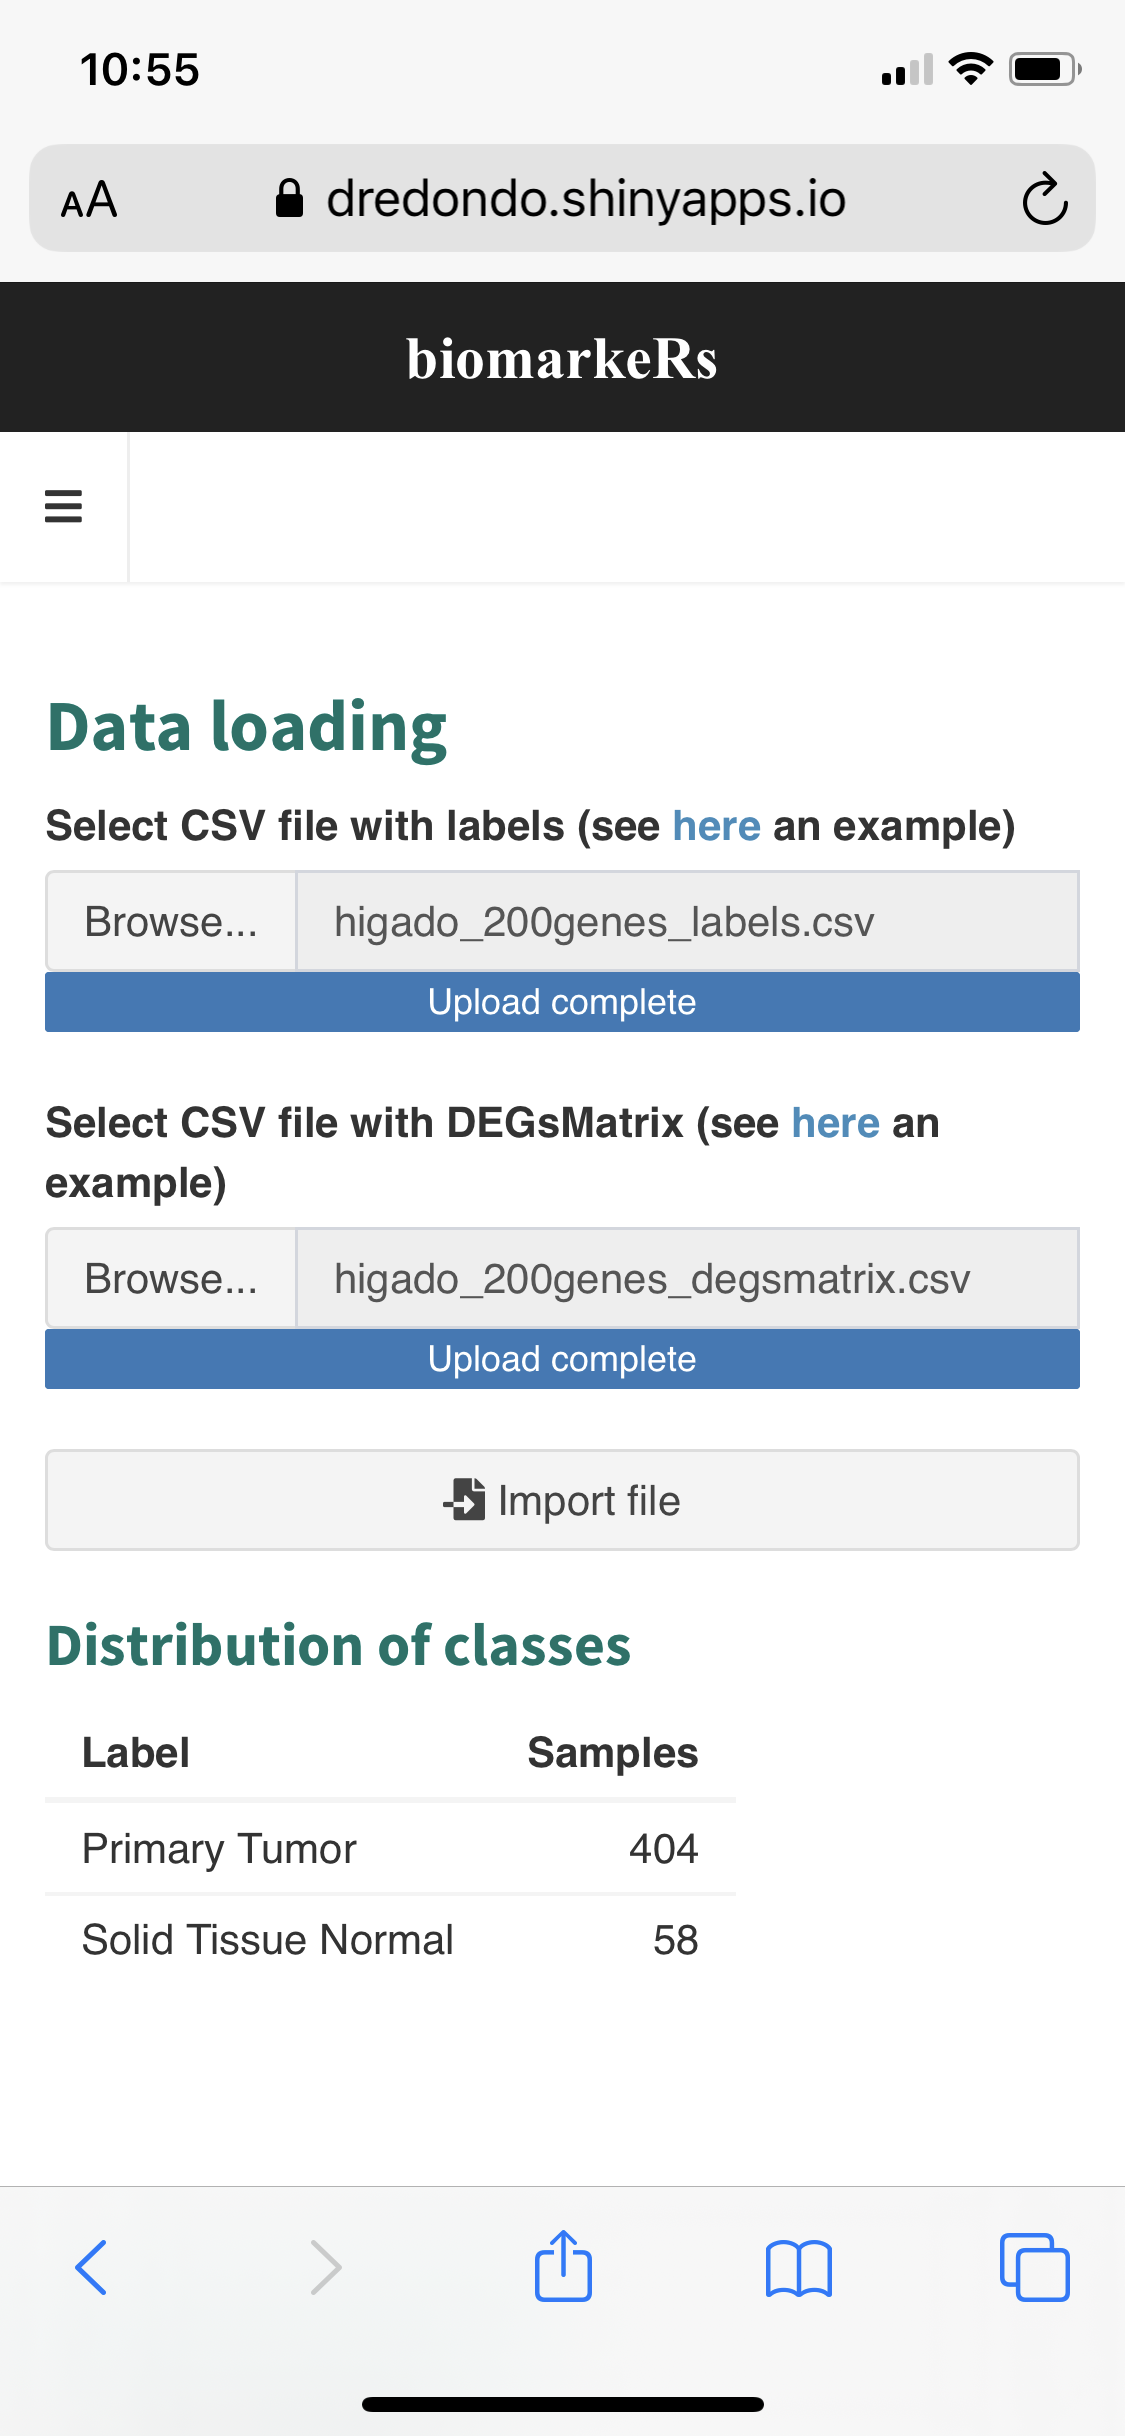
\includegraphics[width=.75\textwidth]{figuras/52_app_iphone.png}
		\end{minipage}%
		\begin{minipage}{.5\textwidth}
			\centering			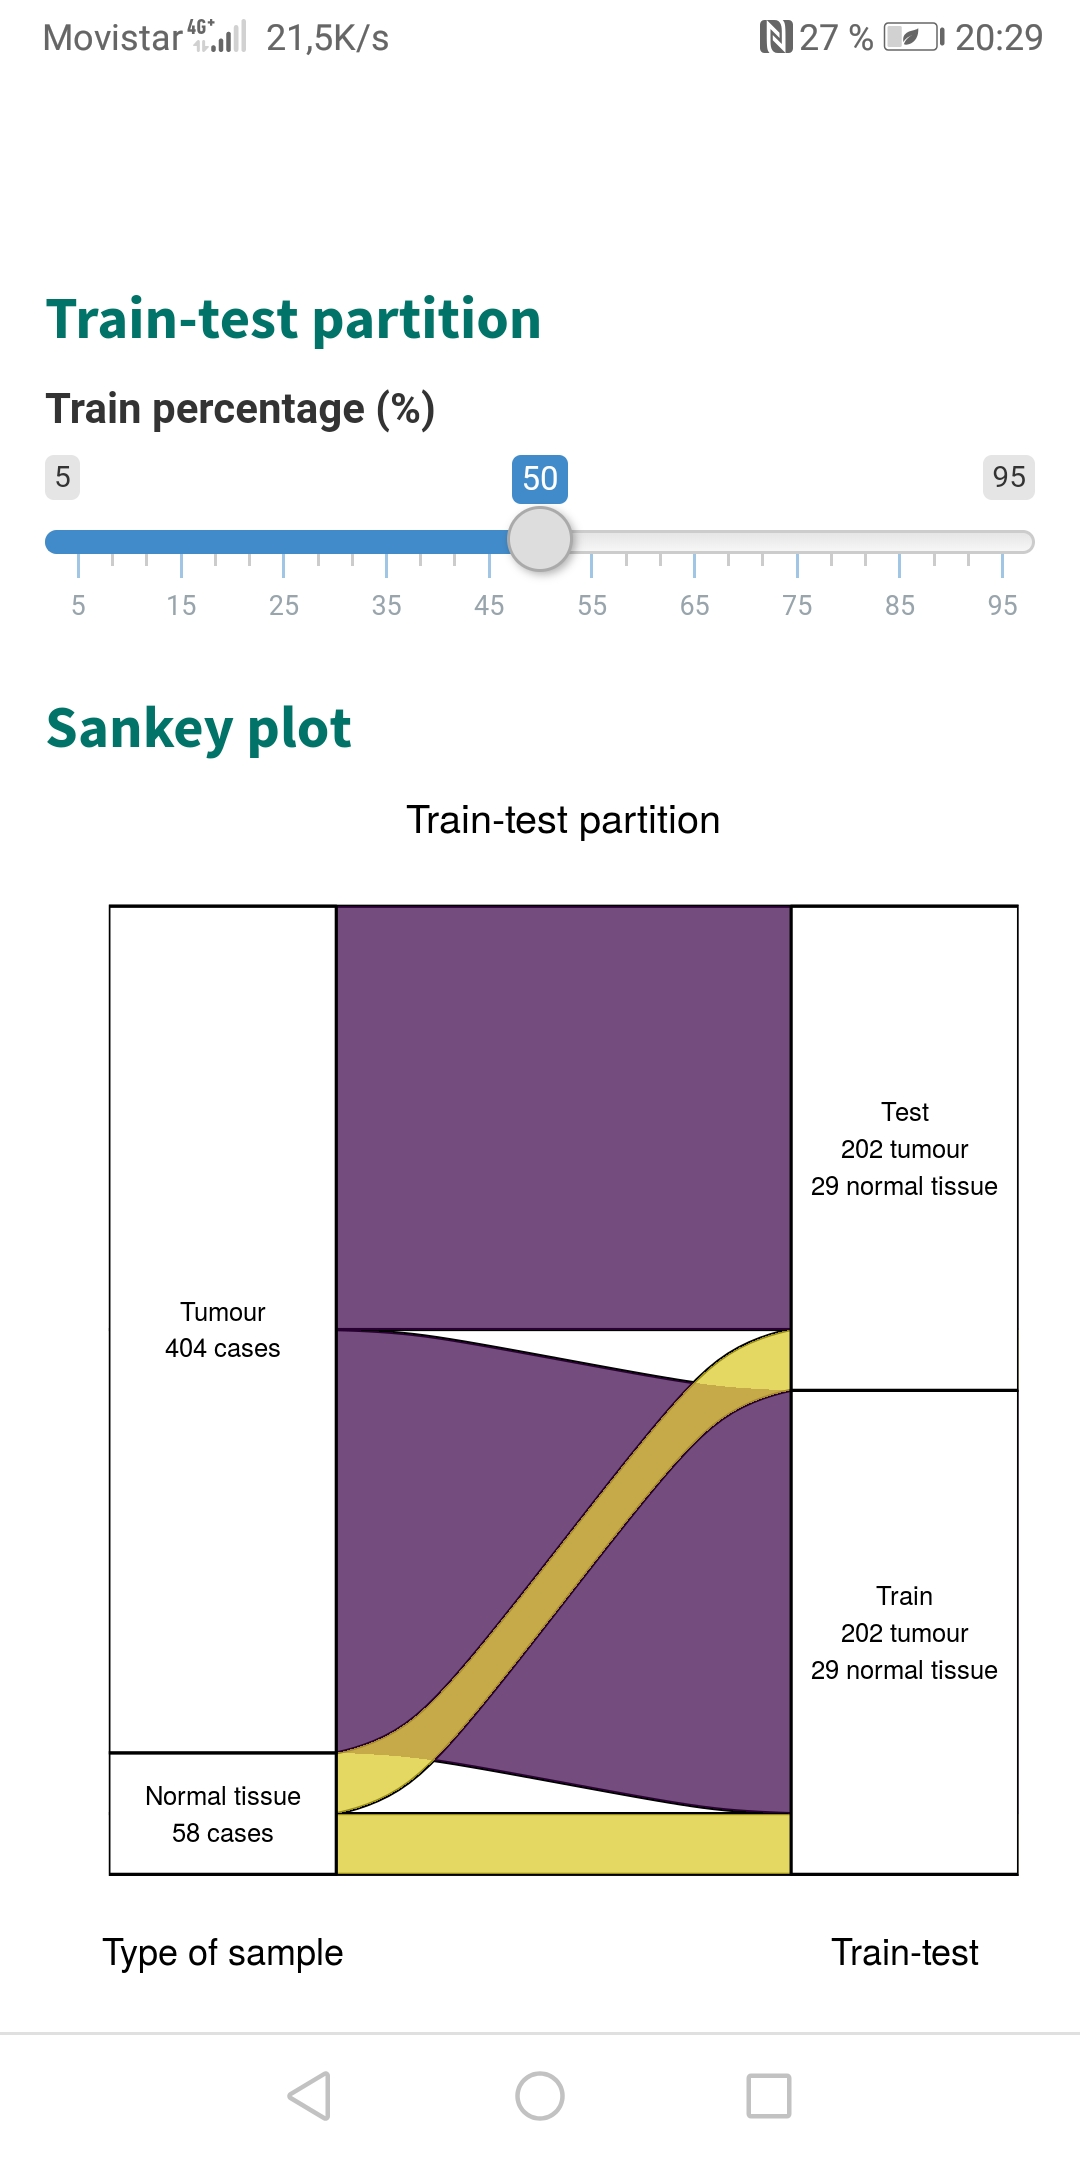
\includegraphics[width=.825\textwidth]{figuras/52_app_huawei.jpg}
		\end{minipage}
	\end{figure}
\end{center}

Para poder ejecutar la aplicación de forma local en un ordenador es necesario tener instalado una versión de R, de RStudio, y de todos los paquetes asociados a la aplicación. Además, puede haber problemas de compatibilidad entre los distintos paquetes. Este inconveniente no es tal en la versión web, gracias a que al realizar el despliegue a la web de la aplicación se realizan copias de las versiones de todos los paquetes que usa la aplicación Shiny localmente \cite{Shinyapps.ioteam2020}. De esta forma se asegura la estabilidad total de la versión web.\\

La versión local puede ser más útil que la versión web en algunas situaciones. Evidentemente, la versión local es mejor alternativa cuando no hay conexión a internet o la conexión es lenta o inestable. Por otra parte, uno de los aspectos en los que la versión local podría mejorar a la versión web es en el coste computacional. La cuenta \textit{premium} de \url{https://www.shinyapps.io/} en la que está alojada la aplicación web permite hasta 8GB de RAM, característica que puede resultar insuficiente para el procesamiento de grandes cantidades de datos transcriptómicos. Otra posible limitación de la versión web es que el tipo de cuenta dispone de un límite de 500 horas/mes de procesamiento. En el caso de alcanzar el límite, se podría mejorar el tipo de cuenta hasta alcanzar las 10.000 horas mensuales. 